\documentclass[12pt]{report}
\usepackage{mioStile}

\pgfplotsset{compat = 1.18}

\title{Teoria dei grafi}
\author{Andrea Cosentino}
\sectionfont{\fontsize{12}{15}\selectfont}
\date{\today}

\begin{document}

\maketitle

\tableofcontents
\setlength{\columnsep}{0.8cm}
\setlength{\columnseprule}{0.2pt}
\twocolumn

\chapter{Prima lezione}
\noindent
Un grafo $G = (V,E)$ è una struttura algebrica dove $V$ è l'insieme finito di vertici e $E$ è l'insieme finito di archi. Inoltre, vale che $E = [V]^2$. Dato un insieme $S$ e un qualunque intero $k \in \{2,\dots,|S|\}$, diciamo che $[S]^k$ è la collezione di tutti i sottoinsieme di $S$ formati da $k$ elementi. Per esempio, dato l'insieme $S = \{1,2,3\}$ l'insieme $[S]^2$ contiene $\{\{1,2\}, \{1,3\},\{2,3\}\}$. 

\begin{exmp}
    Un esempio di grafo $G = (V,E)$ è $V = \{1,2,3\}$ e $E = \{\{1,2\},\{1,3\}\}$.
    
\vspace{10px}
\begin{center}
\begin{tikzpicture}{}
    \node[] (A) {$1$};
    \node[below left= 2cm and 1cm of A] (B){$2$};
    \node[below right= 2cm and 1cm of A] (C){$3$};

    \draw[] (A) -- (B);
    \draw[] (A) -- (C);
\end{tikzpicture}
\end{center}
\end{exmp}

\noindent
Notare che ci concentriamo su grafi con archi non orientati.

La nomenclatura che utilizzeremo per indicare dei vertici generici è $i,j,u,v$, mentre per indicare degli archi generici è $(i,j)$. Dire $(i,j)$ implicherebbe un ordine, per evitare di scrivere $\{i,j\}$ useremo $(i,j)$ senza implicare che l'arco sia orientato.

Il numero di nodi del grafo è detto \textbf{ordine}, e corrisponde a $|V|$. Un grafo di ordine $0$ è detto grafo \textbf{vuoto}, mentre un grafo di ordine $\leq 1$ è detto grafo \textbf{banale}. Esistono solamente due grafi di ordine $2$:

\disegna{ 
    \node[]  (A1) at (-3.5,0) {$A)$};
    \node[nodo] (A) at (-3,0){};
    \node[nodo] (B) at (-1,0){};

    \node[]  (A2) at (-3.5,-2) {$B)$};
    \node[nodo] (C) at (-3,-2){};
    \node[nodo] (D) at (-1,-2){};
    \draw[] (C) -- (D);
}

\noindent
Dato un arco $e = (i,j) \in E$ diciamo che $i,j$ sono vertici incidenti all'arco $e$. Due vertici $i,j$ con $i \neq j$ tali che $(i,j) \in E$ sono detti vertici \textbf{adiacenti} in $G(V,E)$.  Se $E \equiv [V]^2$ diciamo che il grafo è \textbf{completo} oppure che è una \textbf{clique} (o cricca in italiano). Un grafo completo su $n$ vertici è chiamato $K_n$. Alcuni esempi di grafi completi sono

\disegna{

    \node[]  (A) at (2,0) {$K_2$};
    \node[nodo] (A1) at (-2,0){};
    \node[nodo] (A2) at (0,0){};
    \draw[] (A1) -- (A2);

    \node[]  (B) at (2,-3) {$K_3$};
    \node[nodo] (B1) at (-1,-2){};
    \node[nodo] (B2) at (-2,-4){};
    \node[nodo] (B3) at (0,-4){};
    \draw[] (B1) -- (B2);
    \draw[] (B2) -- (B3);
    \draw[] (B1) -- (B3);

    \node[]  (C) at (2,-7) {$K_4$};
    \node[nodo] (C1) at (-2.5,-6){};
    \node[nodo] (C2) at (-2.5,-8){};
    \node[nodo] (C3) at (0.5,-6){};
    \node[nodo] (C4) at (0.5,-8){};
    \draw[] (C1) -- (C2);
    \draw[] (C2) -- (C3);
    \draw[] (C1) -- (C3);
    \draw[] (C1) -- (C4);
    \draw[] (C3) -- (C4);
    \draw[] (C2) -- (C4);
}

\noindent 
Un grafo completo su $n$ vertici ha un numero di archi pari a 
$$\binom{n}{2} = \frac{(n)(n-1)}{2}$$
I grafi che consideriamo sono non orientati e \textbf{semplici}. Un grafo è semplice  se non ha loops (o cappi)

\disegna{
 \node[nodo](A){};
 \node at (1,0) (here){};
 \draw[->,>= stealth]  (A) edge [out=90,in=30,distance=10mm]   (A);
}

\noindent 
e non ha archi multipli, ovvero tra due nodi o c'è un arco non ce n'è neanche io. Quindi la situazione in figura non è ammessa.

\disegna{
 \node[nodo](A){};
 \node[nodo, right =of A] (B){};
 \draw[>= stealth]  (A) edge [out=60,in=150,distance=3.5mm]   (B);
 \draw[>= stealth]  (B) edge [out=-150,in=-60,distance=5mm]   (A);
}

\noindent 
Il sotto-grafo di un grafo $G = (V,E)$ è $G' =(V',E')$ tale che $V' \subseteq V$ e $E' \subseteq E \and [V']^2$. Nella seconda condizione imponiamo che se vogliamo avere l'arco $(i,j)$ nel grafo, allora $i,j \in V'$. Senza questa condizione non otterremmo un grafo. 

\begin{exmp}
    Dato il grafo 
    \disegna{
    \node[nodo] (C1) at (-2.5,-6){};
    \node[left=0.15cm] at (C1.east) {$1$}; 
    \node[nodo] (C2) at (-2.5,-8){};
    \node[left=0.15cm] at (C2.east) {$3$}; 
    \node[nodo] (C3) at (0.5,-6){};
    \node[right=0.15cm] at (C3.west) {$2$}; 
    \node[nodo] (C4) at (0.5,-8){};
    \node[right=0.15cm] at (C4.west) {$4$}; 
    \draw[] (C1) -- (C2);
    \draw[] (C1) -- (C3);
    \draw[] (C3) -- (C4);
    \draw[] (C2) -- (C4);
    }
    Se la seconda condizione fosse solamente $E' \subseteq E$ potremmo scegliere $V' = \{1,2\}$ ed $E' = \{(1,2), (2,3)\}$, ma siccome $3$ non è un nodo, il risultato non è un grafo.
    Un esempio di sotto-grafo è $V' = \{1,2,3,4\}$, $E' = \{(3,4)\}$

    \disegna{
    \node[nodo] (C1) at (-2.5,-6){};
    \node[left=0.15cm] at (C1.east) {$1$}; 
    \node[nodo] (C2) at (-2.5,-8){};
    \node[left=0.15cm] at (C2.east) {$3$}; 
    \node[nodo] (C3) at (0.5,-6){};
    \node[right=0.15cm] at (C3.west) {$2$}; 
    \node[nodo] (C4) at (0.5,-8){};
    \node[right=0.15cm] at (C4.west) {$4$}; 
    \draw[] (C2) -- (C4);
    }

    \noindent 
\end{exmp}

\noindent
Dato $V' \subseteq V$ il sotto-grafo $G'$ \textbf{indotto} da $V'$ è $G'(V',E')$ con $E' = E \and [V']^2$. Ovvero, se seleziono i vertici seleziono anche gli archi su cui sono incidenti. Dato l'insieme di vertici $V'$ c'è solo un sotto-grafo indotto.


Dato il grafo $G(V,E)$ il vicinato di $N(v)$ di $v \in v$ in $G$ è 

$$N(v) = \{j \in V: (v,j) \in E\}$$
Cioè tutti i nodi connessi a $v$ con un arco.

\begin{exmp}
Dato il grafo 
    \disegna{
    \node[nodo] (C1) at (-2.5,-6){};
    \node[left=0.15cm] at (C1.east) {$u$}; 
    \node[nodo] (C2) at (-2.5,-8){};
    \node[left=0.15cm] at (C2.east) {$v'$}; 
    \node[nodo] (C3) at (0.5,-6){};
    \node[above right=0.075cm] at (C3.north east) {$v$}; 
    \node[nodo] (C5) at (2.5,-6){};
    \node[nodo] (C4) at (0.5,-8){};
    \node[right=0.15cm] at (C4.west) {$\omega$}; 
    \draw[] (C1) -- (C2);
    \draw[] (C1) -- (C3);
    \draw[] (C3) -- (C4);
    \draw[] (C2) -- (C4);
    \draw[] (C5) -- (C3);
    \draw[] (C4) -- (C5);
    }
    Il vicinato di $v$ è $N(v) = V \backslash \{v\}$ mentre il vicinato di $v'$ è $N(v') = \{u,v,\omega\}$.
\end{exmp}

\noindent
Il grado di $v$ in $G$ è $d(v) = |N(v)|$. Se $v$ ha $d(v) = 0$ in $G$ allora si dice \textbf{isolato}.

\disegna{
   \node[]  (B) at (2,-4) {$ISOLATO$};
   \node[nodo] (I) at (2,-3){};
    \node[nodo] (B1) at (-1,-2){};
    \node[nodo] (B2) at (-2,-4){};
    \node[nodo] (B3) at (0,-4){};
    \draw[] (B1) -- (B2);
    \draw[] (B2) -- (B3);
    \draw[] (B1) -- (B3);
    \draw[->,>= stealth]  (B) edge [out=60,in=-60,distance=10mm]   (I);
}

\noindent 
Definiamo il grado minimo come $$\delta(G) = \min {d(v): v \in V}$$ e il grado massimo $$\Delta(G) = \max \{d(v) : v \in V\}$$ Se $\Delta(G) = \delta(G) = k$ allora $G$ è $k$-regolare.

\begin{exmp}
    Il seguente grafo è $2$-regolare
    \disegna{
    \node[nodo] (C1) at (-2.5,-6){};
    \node[nodo] (C2) at (-2.5,-8){};
    \node[nodo] (C3) at (0.5,-6){}; 
    \node[nodo] (C4) at (0.5,-8){};
    \node[nodo] (C5) at (-1,-5){};
    \node[nodo] (C6) at (-1.75,-9){};
    \draw[] (C1) -- (C2);
    \draw[] (C1) -- (C5);
    \draw[] (C5) -- (C3);
    \draw[] (C3) -- (C4);
    \draw[] (C2) -- (C6);
    \draw[] (C4) -- (C6);
    }
\end{exmp}

\noindent 
Il grado medio è
$$D(G) = \frac{1}{|V|} \sum_{v \in V} d(v)$$
Vale che $\delta(G) \leq D(G) \leq \Delta(G)$. La \textbf{densità} è invece definita come 

$$\varepsilon(G) = \frac{|E|}{|V|}$$
La densità ci dice quanti archi ha ,in media, ciascun vertice. Assomiglia al grado medio ma in quest'ultimo contiamo due volte ogni arco. Infatti vale che 

$$|E| = \frac{1}{2} \sum_{v \in V} d(v)$$
$$= \frac{1}{2} D(G) |V|$$
e quindi

$$\varepsilon(G) = \frac{|E|}{|V|}  = \frac{1}{2} D(G) $$

\begin{fatto}
In ogni grafo il numero di vertici di grado dispari è pari.
\end{fatto}

\begin{dimo}
    Cominciamo con l'osservare che $|E|$  è un numero intero, e siccome vale che  $|E| = \frac{1}{2} \sum_{v \in V}$ $d(v)$ allora anche $\frac{1}{2} \sum_{v \in V} d(v)$ è intero. Il valore $\sum_{v \in V} d(v)$ deve essere per forza pari, dato che la sua metà è intera. Dividiamo la sommatoria in due sommatorie:
\begin{align*}
\sum_{v \in V:\, d(v) \; \text{è pari}} d(v)  \\ + \sum_{v \in V:\, d(v) \; \text{è dispari}} d(v)
    \end{align*}
    La sommatoria pari ha come risultato sicuramente un numero pari. Questo vuol dire che, se come risultato finale vogliamo un numero pari, anche la sommatoria dispari deve risultare pari. Ciò è possibile se e solo se il numero di elementi è pari. Infatti, sommando un numero pari di numero dispari otteniamo un numero pari. Quindi il numero di vertici di grado dispari è pari.
\end{dimo}

\noindent 
Ci poniamo adesso la domanda se la densità può scendere sotto il grado minimo. Vediamolo prima con un esempio

\begin{exmp}
    Il seguente grafo 
    \disegna{
    \node[nodo] (C) at (-3,-2){};
    \node[nodo] (D) at (-1,-2){};
    \draw[] (C) -- (D);
    }

    \noindent 
    Ha $\delta(G) = 1$ e $\varepsilon(G) = \frac{1}{2}$, quindi $\delta(G) > \varepsilon(G)$
\end{exmp}

\begin{fatto}
    $\forall G$ con almeno un arco, ha un sotto-grafo indotto $H$ tale che 
    $$\delta(H) > \varepsilon(H) \geq \varepsilon(G) $$
\end{fatto}

\begin{dimo}
    Consideriamo una sequenza di grafi

    $$G = G_0, G_1, G_2, \dots$$
    Dove $G_i = (V_i,E_i)$ e $V_0 \supseteq V_1 \supseteq V_2$, con $G_i$ grafo indotto da $V_i$. Se $V_0(=V)$ ha $v_0$ tale che $d(v_0) \leq \varepsilon(G_0)$ creiamo $V_1 = V_0 \backslash \{v_0\}$. Notiamo che se non esiste $v_0$ che rispetta la condizione, allora 

    $$\forall v \in V d(v) > \varepsilon(G_0)$$
    e quindi $d(G_0) > \varepsilon(G_0)$. In questo caso avremmo già dimostrato il teorema con $H = G$.
    
    Consideriamo adesso $G_1$ indotto da $V_1$ (ricordiamo che $V_1 = V_0 \backslash v$). Iteriamo svolgendo la stessa operazione di prima fino a quando $V_i$ è tale che $\forall v \in V_i \, d(v) > \varepsilon(G_i)$. Notiamo che ci fermeremo prima di svuotare il grafo, infatti arriveremo al caso base 

        \disegna{
    \node[nodo] (C) at (-3,-2){};
    \node[nodo] (D) at (-1,-2){};
    \draw[] (C) -- (D);
    }

    \noindent
    dove sappiamo che vale $\delta(G) > \varepsilon(G)$. Se $G_{i+1}$ viene creato, allora

    $$\varepsilon(G_{i+1}) = \frac{|E_{i+1}|}{|V_{i+1}|}$$
    $$=  \frac{|E_i - d(v_i)|}{|V_i - 1|} \geq  \frac{|E_i - \varepsilon(G_i)|}{|V_i - 1|} $$
    Dove la disuguaglianza vale per la condizione con cui costruiamo il sotto-grafo. 
    $$= \frac{|E_i| - \frac{|E_i|}{|V_i|}}{|V_i - 1} =  \frac{|E_i| |V_i| - |E_i|}{|V_i|(|V_i - 1|)}$$
    dove abbiamo portato a fattore comune il numeratore.
    $$= \frac{|E_i| (|V_i| - 1)}{|V_i|(|V_i - 1|)} = \varepsilon(G_i)$$
    Quindi quando ci fermiamo avremo $G_k$ tale che $$\delta(G_k) > \varepsilon (G_k) \geq \varepsilon(G_0) $$

    
\end{dimo}

\chapter{Seconda lezione}

\noindent
Un \textbf{cammino} di lunghezza $k \geq 0$ in $G = (V,E)$ è un sotto-grafo $P_k$ con $k$ archi e $k+1$ vertici distinti tale che $e_i = (v_{i-1},v_i)$. Indichiamo gli archi con $e_1 \dots e_k$ e i nodi con $v_0,\dots,v_k$.

\disegna{
    \node[cloud,draw,minimum width = 5cm,
    minimum height = 4cm] {};
    \node[nodo] (A) at (1,1){}; 
    \node[] at(1,1.3) {$v_0$};
    \node[nodo] (B) at (1.5,0){}; 
    \node[nodo] (C) at (0.8,-1){}; 
    \node[nodo] (D) at (0,-0.6){}; 
    \node[nodo] (E) at (-2,-0.3){};
    \node[] at(-2,0) {$v_k$};
    \draw[] (A) -- (B) node[above,midway,sloped]{$e_1$};
    \draw[] (B) -- (C)  node[below right,midway]{$e_2$};;
    \draw[] (C) -- (D);
    \draw[] (D) -- (E) node[above,midway]{$e_k$};
}

\noindent 
Usiamo la nuvoletta quando non ci interessa la struttura del grafo. Evidenziamo solo una certa parte.
Nel caso in cui $P_0$ non abbiamo archi nel cammino ma un singolo vertice.

Un \textbf{ciclo} $C_k$ di lunghezza $k \geq 3$ è formato da un cammino $P_{k-1}$ che può essere esteso in $G$ includendo l'arco $(v_{k-1},v_0)$.


\disegna{
    \node[cloud,draw,minimum width = 5cm,
    minimum height = 4cm] {};
    \node[nodo] (A) at (1,1){}; 
    \node[] at(1,1.3) {$v_0$};
    \node[nodo] (B) at (1.5,0){}; 
    \node[nodo] (C) at (0.8,-1){}; 
    \node[nodo] (D) at (0,-0.6){}; 
    \node[nodo] (E) at (-2,-0.3){};
    \node[] at(-2,-0.6) {$v_{k-1}$};
    \draw[] (A) -- (B) node[above,midway,sloped]{$e_1$};
    \draw[] (B) -- (C)  node[below right,midway]{$e_2$};;
    \draw[] (C) -- (D);
    \draw[] (D) -- (E) node[above,near start]{$e_{k-1}$};
    \draw[color= red] (E) -- (A) node[above,midway,sloped,color = white] {$(v_{k-1},v_0)$};
}

\noindent 
In un grafo $G$, il \textbf{calibro} $g(G)$ è la lunghezza del ciclo più breve. La \textbf{circonferenza} è la lunghezza del ciclo più lungo. 

\begin{fatto}
    $\forall \; G$ con $\delta(G) > 2$ contiene un cammino di lunghezza $\delta(G)$ e un ciclo di lunghezza almeno $\delta(G) + 1$.
\end{fatto}

\begin{dimo}
    Prendiamo il cammino più lungo del grafo, $P_k$. Allora tutti i vicini di $P_k$ fanno parte del cammino, altrimenti potrei aggiungerli e allungarlo, $P_k$ non sarebbe il più lungo. Quindi il cammino $P_k$ è almeno lungo $|N(v_k)|$, dove $v_k$ è l'ultimo nodo del cammino. Siccome per ipotesi $|N(v_k)| \geq \delta(G)$ allora esiste un cammino di lunghezza  $\delta(G)$.
    Consideriamo ora il primo vertice che è un vicino di $v_k$.

    \disegna{
    \node[cloud,draw,minimum width = 5cm,
    minimum height = 4cm] {};
    \node[nodo] (A) at (1,1){}; 
    \node[] at(1,1.3) {$v_0$};
    \node[nodo, color = blue] (B) at (1.5,0){}; 
    \node[nodo] (C) at (0.8,-1){}; 
    \node[] at(1.8,0) {$v_i$};
    \node[nodo] (D) at (0,-0.6){}; 
    \node[nodo] (E) at (-2,-0.3){};
    \node[] at(-2,-0.6) {$v_{k}$};
    \draw[color = red] (A) -- (B);
    \draw[color = red] (B) -- (C);
    \draw[color = red] (C) -- (D);
    \draw[color = red] (D) -- (E);
    \draw[] (E) -- (B);
    \draw[] (E) edge [out=-60,in=-1200,distance=5mm] (C);
}
In rosso è evidenziato il cammino $P_k$ e in blu il primo vertice che è vicino di $v_k$. Se consideriamo il cammino in rosso da $v_i$ fino a $v_K$ e aggiungiamo $(v_k,v_i)$ troviamo un ciclo, ciò vale sempre per il fatto $\delta(G) \geq 2$. Il ciclo $C$ è lungo almeno $N(v_k) + 1 \geq \delta(G) + 1$.
    
\end{dimo}

\noindent
Dato $G = (V,E)$ $\forall i,j \in V \exists d(i,j)$ se $i,j$ sono connessi in $G$ da almeno $1$ cammino allora $d(i,j)$ è la lunghezza del cammino più breve, altrimenti è $\infty$. 

\begin{exmp}
Dato il grafo
\disegna{
     \node[cloud,draw,minimum width = 2.5cm,
    minimum height = 4cm] at(-2,0) {};
    \node[cloud,draw,minimum width = 2.8cm,
    minimum height = 4cm] at(2,0) {};

    \node[nodo] at(-1.8,0.3){};
    \node[nodo] at(2.3,-0.5){};
    \node[] at(-1.8,0.7) {$i$};
    \node[] at(2.3,-0.1) {$j$};
 }
 La distanza tra $i,j$ è $d(i,j) = \infty$.
\end{exmp}

\noindent
Il \textbf{diametro} è definito come

$$diam(G) = \max_{i,j \in V} d(i,j) =  \max_{i \in V}  \max_{j \in V} d(i,j) $$
e il raggio 

$$rad(G) = \min_{i\in V} \max_{j \in V} d(i,j)$$
Il raggio lo possiamo vedere come il punto "più centrale". Sia $x$ questo punto centrale, vale che $\forall v \in V d(x,v) \leq rad(G)$. Inoltre  $rad(G) \leq diam(G)$ e questo è ovvio dato che il diametro è una massimizzazione del massimo, mentre il raggio è una minimizzazione del massimo.
Possiamo anche dire che $diam(G) \leq 2 rad(g)$, dato che 
$$\forall u,v \in V d(u,v) \leq d(u,x) + d(x,v)$$
$$\leq rad(G) + rad(G) = 2 rad(G)$$

\begin{fatto}
    $\forall G$ che ha almeno un ciclo soddisfa

    $$g(G) \leq 2 diam(G) + 1$$
\end{fatto}

\noindent
\begin{dimo}
    Consideriamo il grafo
    \disegna{
    \node[cloud,draw,minimum width = 5cm,
    minimum height = 4cm] {};
    \node[nodo] (A) at (1,1){}; 
    \node[] at(1,1.3) {$x$};
    \node[nodo] (B) at (1.5,0){}; 
    \node[nodo] (C) at (0.8,-1){}; 
    \node[nodo] (D) at (0,-0.6){}; 
    \node[nodo] (E) at (-2,-0.3){};
    \node[nodo] (F) at (-1.4,0){};
    \node[nodo] (G) at (0,0.2){};
    \node[nodo] (H) at (0.2,1.2){};
    \node[] at(-2,-0.6) {$y$};
    \draw[color = red] (A) -- (B);
    \draw[color = red] (B) -- (C);
    \draw[color = red] (C) -- (D);
    \draw[color = red] (D) -- (E);
    \draw[color = blue] (E) -- (F);
    \draw[color = blue] (F) -- (G);
    \draw[color = blue] (G) -- (H);
    \draw[color = blue] (H) -- (A);
}
dove il ciclo $C$ è il più corto, con lunghezza $g(G)$. I due vertici $x,y$ sono vertici opposti, cioè tagliano il ciclo in due parti il più possibile uguali. Chiamiamo il percorso in rosso $p_1$ e il percorso in blu $p_2$. Assumiamo per assurdo che $g(G) \geq 2 diam(G) + 2$. Allora $p_1,p_2$ sono lunghi ciascuno almeno $diam(G) + 1$. Però $d(x,y) \leq diam(G)$ per la definizione stessa di diametro. Non tutti gli archi di $P$ (cioè del percorso più breve) stanno su $C$, altrimenti il ciclo avrebbe lunghezza $2diam(G) + 1$. Quindi, possiamo costruire un ciclo più piccolo, prendendo gli archi che non stanno né su $P_1$ né su $P_2$.

 \disegna{
    \node[cloud,draw,minimum width = 5cm,
    minimum height = 4cm] {};
    \node[nodo] (A) at (1,1){}; 
    \node[] at(1,1.3) {$x$};
    \node[nodo] (B) at (1.5,0){}; 
    \node[nodo] (C) at (0.8,-1){}; 
    \node[nodo] (D) at (0,-0.6){}; 
    \node[nodo] (E) at (-2,-0.3){};
    \node[nodo] (F) at (-1.4,0){};
    \node[nodo] (G) at (0,0.2){};
    \node[nodo] (H) at (0.2,1.2){};
    \node[] at(-2,-0.6) {$y$};
    \draw[color = red] (A) -- (B);
    \draw[color = orange] (B) -- (C);
    \draw[color = orange] (C) -- (D);
    \draw[color = orange] (D) -- (E);
    \draw[color = blue] (E) -- (F);
    \draw[color = blue] (F) -- (G);
    \draw[color = blue] (G) -- (H);
    \draw[color = blue] (H) -- (A);
    \draw[color = orange, dashed] (E) -- (B);
}

\noindent 
Il ciclo in arancione è più piccolo di $C$, quindi deve per forza valere che $g(G) \leq 2 diam(G) + 1$.
\end{dimo}

\section{Connettività di un grafo}
Un grafo è \textbf{sconnesso} se $\exists i,j \in V$ $|\; d(i,j) = \infty$. Una \textbf{componente} di un grafo è un qualunque insieme massimale di vertici connessi. Se un grafo è connesso il componente è il grafo stesso. $G$ è $k$-connesso se $|V| > k$ e $\forall X \subset V$ con $|X| < k$ il sotto-grafo indotto $V \backslash X$ è connesso.  Se un grafo è $k$-connesso non possiamo sconnettere il grafo rimuovendo al più $k-1$ vertici. Tutti i grafi sono $0$-connessi. Se $G$ è connesso è anche $1$-connesso, tranne il caso $K_1$ (cricca di un elemento) perché non rispetta la condizione $|V| > 1$. Il massimo intero $k$ tale che $G$ è k-connesso è detta \textbf{connettività} di $G$, che denotiamo con $K(G)$. Vale che $K(K_n) = n-1$.

\begin{exmp}
    Nel caso di $K_4$
    \disegna{
        \node[nodo] (C1) at (-2.5,-6){};
    \node[nodo] (C2) at (-2.5,-8){};
    \node[nodo] (C3) at (0.5,-6){};
    \node[nodo] (C4) at (0.5,-8){};
    \draw[] (C1) -- (C2);
    \draw[] (C2) -- (C3);
    \draw[] (C1) -- (C3);
    \draw[] (C1) -- (C4);
    \draw[] (C3) -- (C4);
    \draw[] (C2) -- (C4);
    }
    il numero di nodi che possiamo rimuovere è $3$.
\end{exmp}

\begin{teo}
    Se $G \notin \{k_0,k_1\}$ (ovvero $G$ non è un grafo banale), allora $K(G) \leq F \leq \delta(G)$ dove $k$ è qualsiasi insieme minimo di archi la cui rimozione sconnette il grafo.
\end{teo}

\begin{dimo}
    La disequazione $F \leq \delta(G)$ è banale. Infatti se sconnetto tutti gli archi attorno a un nodo ho sconnesso il grafo. Concentriamoci su $K(G) \leq F$ e distinguiamo due casi:

    \begin{itemize}
        \item $G$ ha un vertice $v$ che non è incidente a $F$.
    \end{itemize}
                    \disegna{
     \node[cloud,draw,minimum width = 2.5cm,
    minimum height = 4cm] at(-2,0) {};
    \node[cloud,draw,minimum width = 2.8cm,
    minimum height = 4cm] at(2,0) {};

    \node[nodo] (A) at(-1.6,0.9){};
    \node[nodo] (A1) at(-1.55,0.3){};
    \node[nodo] (A2) at(-1.65,-0.3){};
    \node[nodo] (A3) at(-1.6,-0.9){};
    \node[nodo] (v) at(-2.5,0){};
    \node[] at (-2.5,0.3){$v$};
    \node[nodo] (B) at(1.6,0.9){};
    \node[nodo] (B1) at(1.65,0.3){};
    \node[nodo] (B3) at(1.60,-0.9){};
    \draw[] (A)--(B1);
    \draw[] (A1)--(B);
    \draw[] (A2) -- (B3);
    \draw[] (A3) -- (B3);
    \draw (-1.5,0) ellipse (0.5cm and 2cm);
    \draw (0,0) ellipse (0.5cm and 1.5cm);
    \node[] (VC) at (-0.5,-2){$V_c$};
    \node[] (F) at (0,0){$F$};
    \node[] (C) at (-3,-2){$C$};
    \draw[->,>= stealth]  (VC) edge [out=-140,in=-60,distance=7mm]   (-1,-1.85);
     \draw[->,>= stealth]  (C) edge [out=80,in=--150,distance=7mm]   (-2.8,-1.5);
    }

    \noindent 

    dove $C$ è la componente del grafo che ottengo quando rimuovo $F$ e $V_c$ è l'insieme dei nodi connessi agli archi in $F$. Siccome rimuovendo $V_c$ sconnetto il grafo allora $K(G) \leq |V_c| \leq |F|$ 
    \begin{itemize}
        \item $G$ è tale che tutti i vertici sono incidenti con qualche arco in $F$.
    \end{itemize}
    \disegna{
     \node[nodo] (A1) at(-1.55,0.3){};
     \node[] at (-1.55,0.6){$v$};
    \node[nodo] (A2) at(-1.65,-0.3){};
    \node[nodo] (A3) at(-1.6,-0.9){};
    \node[nodo] (B) at(1.6,0.9){};
    \node[nodo] (B1) at(1.65,0.3){};
    \node[nodo] (B3) at(1.60,-0.9){};
    \draw[] (A1) -- (B1);
    \draw[] (A2) -- (B);
    \draw[] (A3) -- (B3);
    \draw[>= stealth]  (A1) edge [out=120,in=-120,distance=7mm]   (A3);
    \draw[>= stealth]  (B3) edge [out=60,in=-60,distance=7mm]   (B);
    \draw[] (A1) -- (A2);
    \draw[] (A3) -- (A2);
    \draw[] (B) -- (B1);
    \draw[] (B1) -- (B3);
    \draw (0,0) ellipse (0.5cm and 1.5cm);
    \node[] (F) at (0,0){$F$};
    }
    Il grafo $G$ ha connettività $K(G) \leq d(v)$. Siccome $d(v) = |F| = \delta(G)$ vale che $K(G) \leq |F|$.
\end{dimo}

\chapter{Terza lezione}

\section{Cammino euleriano}

\noindent
Un cammino \textbf{chiuso} (in inglese closed walk) è un ciclo in cui i vertici non sono distinti. Un cammino chiuso si dice \textbf{euleriano} se attraversa tutti gli archi del grafo esattaemente una volta. Un grafo è euleriano se ammette un cammino euleriano.

\begin{teo} \textbf{Teorema di Eulero (1746)}

\noindent 
Un grafo connesso è euleriano se e solo se ogni vertice ha grado pari.
\end{teo}

\begin{dimo}
    Cominciamo con dimostrare il lato $=>$ del teorema. Quindi, dato un grafo connesso euleriano questo ogni vertice ha grado pari. Prendiamo un vertice che si trova sul cammino euleriano.
    \disegna{
        \node[nodo] (X) {};
        \node[nodo] (A) at (1,1.5) {};
        \node[nodo] (B) at (1,-1.5) {};
        \node[nodo] (C) at (-1,1.5) {};
        \node[nodo] (D) at (-1,-1.5) {};
        \node[nodo] (E) at (-2,0.75) {};
        \draw[>= stealth]  (X) edge [out=60,in=-60,distance=7mm]   (A);
        \draw[>= stealth]  (X) edge [out=-30,in=110,distance=7mm]   (B);
        \draw[>= stealth]  (X) edge [out=110,in=-30,distance=7mm]   (C);
        \draw[>= stealth]  (X) edge [out=-100,in=60,distance=7mm]   (D);
        \draw[>= stealth, dotted]  (X) edge [out=120,in=60,distance=7mm]   (E);
    }
    \noindent
    Se il cammino passa per il vertice, allora deve sia entrare che uscire. Non può esserci un arco che collega un vicino che non sia nel cammino. Quindi o un vertice è isolato oppure il cammino esce ed entra. Allora devono avere grado pari.
    
    L'altro verso necessita un po' più di lavoro per essere dimostrato. Quello che vogliamo dimostrare è che se ogni vertice ha grado pari allora il grafo è euleriano.  Facciamo una dimostrazione per induzione su $|E|$.

    \noindent 
    \textbf{Caso base} $|E| = 0$, banale. Implica che $|V| = 1$ perché parliamo di grafi connessi.

    \noindent 
    \textbf{Ipotesi induttiva} $|E| \geq  1$. Enunciamo un fatto utile.

    \begin{fatto}
        Se $G$ ha tutti i vertici con grado pari con $E \leq 1$, posso trovare in $G$ un cammino chiuso che non contiene un arco \textbf{più} di una volta. 
    \end{fatto}

    \noindent
    Sia $\omega$ un tale cammino di lunghezza massima. Ne rappresentiamo uno da esempio in figura.
    
    \disegna{
        \node[nodo] (A) at (0,0) {};
        \node[nodo] (B) at (1,1) {};
        \node[nodo] (C) at (2,0) {};
        \node[nodo] (D) at (1,-1) {};
        \node[nodo] (E) at (-1,1) {};
        \node[nodo] (F) at (-1,-1) {};
        \node[nodo] (G) at (-2,0) {};

        \draw[] (A) -- (B);
        \draw[] (A) -- (E);
        \draw[] (A) -- (D);
        \draw[] (A) -- (F);
        \draw[] (B) -- (C);
        \draw[] (C) -- (D);
        \draw[] (G) -- (E);
        \draw[] (G) -- (F);
    }

    \noindent 
    Definiamo come $F$ l'insieme degli archi di $\omega$. Se $F \equiv E$ allora abbiamo finito, dato che tutti gli archi di $G$ fanno parte del cammino $\omega$. Assumiamo per assurdo che non sia così. Allora deve valere $$E' \equiv E \backslash F \neq \varnothing$$ 
    Notiamo che $\forall v \in V$ un numero pari di $u \in N(v)$ appartiene a $F$.  Allora il sotto-grafo $G' = (V,E')$ ha tutti i vertici di grado pari (ricordiamo che $0$ è pari). E' evidente che ci debba essere almeno n nodo $e$ attaccato al cammino, altrimenti il grafo non sarebbe connesso.

        
    \disegna{
        \node[nodo] (A) at (0,0) {};
        \node[nodo] (B) at (1,1) {};
        \node[nodo] (C) at (2,0) {};
        \node[nodo] (D) at (1,-1) {};
        \node[nodo] (E) at (-1,1) {};
        \node[nodo] (F) at (-1,-1) {};
        \node[nodo] (G) at (-2,0) {};
        \node[nodo] (H) at(2,2){};
        \node[] at (2,2.3){$e$}; 
        
        \draw[] (A) -- (B);
        \draw[] (A) -- (E);
        \draw[] (A) -- (D);
        \draw[] (A) -- (F);
        \draw[] (B) -- (C);
        \draw[] (C) -- (D);
        \draw[] (G) -- (E);
        \draw[] (G) -- (F);
        \draw[dashed] (B) -- (H);
    }
    Sia $C$ la componente di $G'$ che contiene $e$. $C$ ha un numero di archi $< |E|$, dato che almeno un arco l'abbiamo rimosso. Per ipotesi induttiva $C$ contiene un cammino euleriano. Ma allora possiamo costruire un cammino euleriano per $G$ unendo $\omega$ e il cammino trovato in $C$. Quindi abbiamo costruito un cammino più lungo di $\omega$, contraddicendo l'ipotesi che sia massimo. Allora $F \equiv E$ e così abbiamo dimostrato il teorema. 
\end{dimo}

\noindent 
Se un grafo è euleriano possiamo trovare un cammino euleriano in tempo $O(|E|)$, i.e. in tempo lineare nella descrizione del grafo (algoritmo di Hierholzer). 

\section{Ciclo hamiltoniano}
Un \textbf{ciclo hamiltoniano} è un ciclo che contiene tutti i vertici.  Un grafo si dice hamiltoniano se contiene un ciclo hamiltoniano. Non è nota alcuna condizione necessarie e sufficiente affinché un grafo sia hamiltoniano. Sono note solamente condizioni sufficienti.

\begin{teo}
    Teorema di Dirac (1952).

    \noindent
    Un grafo $G = (V,E)$ con $|V| \geq 3$ e $\delta(G) \geq \frac{|V|}{2}$ è hamiltoniano. 
\end{teo}

\begin{dimo}
    Cominciamo con dimostrare che $G$ deve essere connesso. Se per assurdo non lo fosse allora ha almeno due componenti. 

    \disegna{
     \node[cloud,draw,minimum width = 2.5cm,
    minimum height = 3cm] at(-2,0) {};
    \node[cloud,draw,minimum width = 2.8cm,
    minimum height = 3cm] at(2,0) {};
 }
    Ogni componente è tale che $|C| \leq \frac{|V|}{2}$. Questo è ovvio, perché se una componente ne avesse più di $\frac{|V|}{2}$, un'altra dovrebbe averne di meno, e quindi non varrebbe la condizione $\delta(G) \geq \frac{|V|}{2}$. Notiamo ora che $$\forall v \in C \; d(v) \leq |C| - 1 $$ poiché al massimo un nodo può avere un arco con tutti gli altri nodi nella componente. Questa affermazione ci porta a poter dire che 
    $$d(v) \leq |C| - 1 < \frac{|V|}{2}$$
    ovvero
    $$d(v) < \frac{|V|}{2}$$
    che viola le ipotesi. 
    Sappiamo che $G$ è connesso. Sia ora $p$ un cammino di lunghezza massima in $G$ con nodi $v_0,v_1,\dots,v_k$, con archi $(v_i,v_{i+1})$, dove $v_i$ viene detto \textbf{vertice sinistro} e $v_{i+1}$ \textbf{vertice destro}.

    \disegna{
        \node[nodo] (A) at (-2,0){};
        \node[] at (-2,0.3){$v_0$};
        \node[nodo] (B) at (-1,0){};
        \node[] at (-1,0.3) {$v_1$};
        \node[nodo] (C) at (0,0){};
        \node[] at (0,0.3) {$v_i$};
        \node[nodo] (D) at (1,0){};
        \node[] at (1,0.3) {$v_{1+1}$};
        \node[nodo] (E) at (2,0){};
        \node[] at (2,0.3) {$v_{k-1}$};
        \node[nodo] (F) at (3,0){};
        \node[] at (3,0.3) {$v_{k}$};

        \draw[] (A) -- (B);
        \draw[dashed] (B) -- (C);
        \draw[] (C) -- (D);
        \draw[dashed] (D) -- (E);
        \draw[] (E) -- (F);
    }

    \noindent 
    Tutti i vicini di $v_0$ e $v_k$ sono nel cammino, altrimenti posso allungarlo aggiungendoli. Ricordiamo che vale anche $d(v_i) \geq \frac{n}{2}$ dove $n = |V|$. $p$ non può avere più di $n$ archi, quindi la sua lunghezza $k$ è tale che
        $$k \leq n-1$$
    dove non può essere $k \geq n$ sennò ripeterei dei nodi (e quindi non sarebbe un cammino). Ora associamo a ogni vicino di $v_0$ l'arco a sinistra (per esempio a $v_i$ associamo $(v_{i-1},v_i)$) e a ogni vicino di $v_k$ l'arco a destra. Per il principio della piccionaia c'è almeno un arco che è preso sia da un vicino di $v_0$ che da un vicino i $v_k$

    \disegna{
        \node[nodo] (A) at (-2,0){};
        \node[] at (-2,0.3){$v_0$};
        \node[nodo] (B) at (-1,0){};
        \node[] at (-1,0.3) {$v_1$};
        \node[nodo] (C) at (0,0){};
        \node[] at (0,0.3) {$v_i$};
        \node[nodo] (D) at (1,0){};
        \node[] at (1,0.3) {$v_{1+1}$};
        \node[nodo] (E) at (2,0){};
        \node[] at (2,0.3) {$v_{k-1}$};
        \node[nodo] (F) at (3,0){};
        \node[] at (3,0.3) {$v_{k}$};

        \draw[color= blue] (A) -- (B);
        \draw[dashed] (B) -- (C);
        \draw[color = orange] (C) -- (D);
        \draw[dashed] (D) -- (E);
        \draw[color = red] (E) -- (F);
        \draw[>= stealth, dashed]  (A) edge [out=-60,in=-120,distance=7mm]   (D);
        \draw[>= stealth, dashed]  (F) edge [out=120,in=60,distance=8mm]   (C);
    }

    \noindent 
    Possiamo costruire un ciclo che va da $v_0$ a $v_i$, poi da $v_i$ raggiunge $v_k$, da $v_k$ a $v_{i+1}$ e poi $v_0$.

    \disegna{
        \node[nodo] (A) at (-2,0){};
        \node[] at (-2,0.3){$v_0$};
        \node[nodo] (B) at (-1,0){};
        \node[] at (-1,0.3) {$v_1$};
        \node[nodo] (C) at (0,0){};
        \node[] at (0,0.3) {$v_i$};
        \node[nodo] (D) at (1,0){};
        \node[] at (1,0.3) {$v_{1+1}$};
        \node[nodo] (E) at (2,0){};
        \node[] at (2,0.3) {$v_{k-1}$};
        \node[nodo] (F) at (3,0){};
        \node[] at (3,0.3) {$v_{k}$};

        \draw[color= blue] (A) -- (B);
        \draw[dashed, color = blue] (B) -- (C);
        \draw[] (C) -- (D);
        \draw[dashed, color = red] (D) -- (E);
        \draw[color = red] (E) -- (F);
        \draw[>= stealth, color = red]  (A) edge [out=-60,in=-120,distance=7mm]   (D);
        \draw[>= stealth, color = blue]  (F) edge [out=120,in=60,distance=8mm]   (C);
    }

    \noindent 
    Se esistesse un vertice che non facesse parte di questo ciclo, sarebbe sicuramente un vicino, dato che il grafo è connesso. Ma allora potrei usarlo per allungare il percorso $p$ violando l'ipotesi di massimalità. Quindi il ciclo passa per tutti i nodi, i.e. è hamiltoniano.
    
\end{dimo}

\noindent
Il problema di determinare se un grafo $G$ contenga un cammino hamiltoniano è  NP-completo, questo spiega  il motivo per cui non c siano delle condizioni necessarie e sufficienti. 

\section{Grafo bipartito}
Un grafo $G = (V,E)$ è detto \textbf{bipartito} se $\exists $ una partizione $V_1,V_2$ di $V$ tali che $\forall (i,j) \in E \; i \in V_1 \land j \in V_2$ o viceversa.
Ricordiamo che $V_1$ e $V_2$ in quanto partizione di $V$ sono tali che $V_1 \cap V_2 \equiv  $ $V_1 \cup V_2 = \varnothing$.

\begin{exmp}
    I grafi bipartiti sono usati per esempio su Tinder, Amazon e Netflix.

    \disegna{
    \node[nodo] (A) at(-1.6,0.9){};
    \node[nodo] (A1) at(-1.6,0.3){};
    \node[nodo] (A2) at(-1.6,-0.3){};
    \node[nodo] (A3) at(-1.6,-0.9){};
    \node[nodo] (B2) at(1.6,0.9){};
    \node[nodo] (B) at(1.6,0.3){};
    \node[nodo] (B1) at(1.6,-0.3){};
    \node[nodo] (B3) at(1.60,-0.9){};
    \draw[] (A)--(B1);
    \draw[] (A1)--(B);
    \draw[] (A2) -- (B3);
    \draw[] (A3) -- (B3);
    \draw[] (A3) -- (B2);
    \draw (-1.5,0) ellipse (0.5cm and 2cm);
    \draw (1.5,0) ellipse (0.5cm and 2cm);
    \node[] (V1) at (-0.5,-2){$V_1$};
    \draw[->,>= stealth]  (V1) edge [out=-140,in=-60,distance=7mm]   (-1,-1.85);
    \node[] (V2) at (0.5,-2){$V_2$};
    \draw[->,>= stealth]  (V2) edge [out=-60,in=-140,distance=7mm]   (1,-1.85);
    }

    \noindent 
    Possono contenere cicli, che sono sempre pari! Vale anche il viceversa, ovvero un grafo che contiene solo cicli di lunghezza pari è bipartito.
\end{exmp}


\chapter{Quarta lezione}
\section{Parametri dei grafi}

Possiamo definire informalmente un \textbf{parametro} come una proprietà. Ne abbiamo già viste alcune: 

\begin{itemize}
    \item Taglia
    \item Numero di lati
    \item Diametro
    \item Calibro
\end{itemize}
Formalmente un parametro è una funzione 

$$\phi: \mathscr{G} \rightarrow \mathbf{R}$$
dove $\mathscr{G}$ è la classe dei grafi non orientati e semplici. Altre possibili proprietà possono essere:

\begin{itemize}
    \item $G$ è euclideo?
    \item $K_3 \subseteq G$?
\end{itemize}
I parametri sono detti \textbf{invarianti}, ovvero mantengono lo stesso valore tra \textbf{isomorfismi} di grafi. 
\begin{defi}
    Dati due grafi $G,H \in \mathscr{G}$ sono isomorfismi se $\exists f: V(G) \rightarrow V(H)$ con $f$ biettiva tale che  $$\{(x,y)\} \in E(G) \Longleftrightarrow \{f(x),f(y)\} \in E(H)$$
    $f$ è detto isomorfismo tra $G$ e $H$.
\end{defi}

\noindent
Tutti i $\phi$ sono isomorfismi.

\subsection{Numero di indipendenza}

\begin{defi}
    $U \subseteq V$ è indipendente in $G = (V,E)$ se $$\forall x,y \in U \{x,y\} \notin E$$
    In altre parole $G[U] = (V,\varnothing)$ è un grafo privo di lati.
\end{defi}

\begin{defi}
    $\alpha(G)$ è detto \textbf{numero di indipendenza} ed è tale che
    \begin{multline*}
    \alpha(G) := \max\{k \in \mathbb{N} | \exists U \subseteq V \; \\ \text{indipendente in }\;  G  \land |U|= k \}
    \end{multline*}

\end{defi}

\noindent
Il problema di trovare il numero di indipendenza maggiore è NP-completo.  Notiamo che $\alpha(G)$ sommato alla dimensione più piccola di vertex cover in $G$ è uguale a $|V|$.

\disegna{

\node[cloud,draw,minimum width = 2.5cm,
    minimum height = 3cm] at (-2,0) {};

\node[cloud,draw,minimum width = 2.5cm,
    minimum height = 3cm] at (2,0) {};
\node[] at (-2,2) {$U$};
\node[] at (2,2) {$V \backslash U$};
\node[nodo] (A) at (1.8,-0.4) {};
\node[nodo] (B) at (2.2,0.2) {};
\node[nodo] (C) at (1.5,0.5) {};
\draw (A) -- (B);
\draw (B) -- (C);
\node[nodo] (D) at (-1.8,0.1){};
\node[nodo] (E) at (-2.4,0.8){};
\draw (A) -- (D);
\draw (C) -- (D);
\draw (E) -- (B);
}

\noindent 
Notiamo infatti che i nodi in $U$ hanno almeno un arco con un nodo in $V\backslash U$, altrimenti il grafo sarebbe sconnesso. Notiamo anche che, per definizione, i nodi in $U$ non sono collegati tra loro. Inoltre, ogni nodo in $V\backslash U$ è collegato ad almeno un nodo in $U$, altrimenti $U$ non sarebbe massimale. E' quindi evidente che per coprire tutti gli archi ho bisogno  di tutti i nodi di $V\backslash U$. Assumiamo per assurdo che non sia così, e ci sia un nodo $\omega$ di $V \backslash U$ che non usiamo. Allora gli archi tra $\omega$ e $U$ non sono coperti. Per metterci in un caso favorevole assumiamo anche che gli archi $(j,\omega) \in E$ tali che $j \in V \backslash U $ siano già coperti da $j$ (se così non fosse avremmo bisogno di $\omega$ per coprirli e quindi avremmo dimostrato la sua necessità). I nodi in $i \in U$ tali che $(i,\omega) \in E$ devono essere parte della vertex cover, altrimenti non copriamo degli archi. Tuttavia, se invece di scegliere $\omega$ scegliamo $i$, la cardinalità resterebbe la stessa. Ma se $i$ coprisse due archi, $(i,\omega)$ e $(i,\omega_1)$ tale che $\omega_1 \in V \backslash U$, allora potremmo scegliere $i$ per coprirli entrambi, ottenendo una cardinalità minore. Ma se $\omega,\omega_1$ hanno altri archi con nodi in $U$, allora questi sarebbero scoperti, e andrebbero coperti aggiungendo dei nodi, vanificando il vantaggio ottenuto. Se però non ne hanno altri allora $\omega,\omega_1$ formano, insieme a $U \backslash i$ un insieme indipendente più grande, e ciò non è possibile.

\subsection{Numero di clique}

\begin{defi}
    Il \textbf{numero di clique} è definito come 
    \begin{multline*}
        \omega(G) := \max\{k \in \mathbb{N} | \exists U \subseteq V,\\ G[U] \; \text{completo con} \; |U| = k\}
    \end{multline*}
\end{defi}

\noindent 
Il problema di trovare il numero di cricca massimo è NP-completo. Una cricca in $G =(V,E)$ è un insieme indipendente in $\bar G$ ($G$ \textbf{complemento}), dove $\bar G$ è definito come 

$$\bar G = (V , [V]^2 \backslash E)$$

\begin{exmp} In figura $G$ e il suo complemento.
    \disegna{
        \node[nodo] (A) at (-3,1) {};
        \node[nodo] (B) at (-3,-1) {};
        \node[nodo] (C) at (-1,1) {};
        \node[nodo] (D) at (-1,-1) {};
        \draw[] (C) -- (B);
        \draw[] (A) -- (C);
        \draw[] (B) -- (D);
        \draw[] (D) -- (C);
        \node[nodo] (A1) at (1,1) {};
        \node[nodo] (B1) at (1,-1) {};
        \node[nodo] (C1) at (3,1) {};
        \node[nodo] (D1) at (3,-1) {};
        \draw[] (A1) -- (B1);
        \draw[] (A1) -- (D1);
    }
\end{exmp}

\subsection{Numero cromatico}

\begin{defi}
    Una \textbf{coloratura} dei vertici $G=(V,E)$ è una funzione
    $$c\;:\; V \rightarrow \{1,\dots,k\}$$
    tale che $\{x,y\} \in E \Rightarrow c(x) \neq c(y)$.
\end{defi}
 La funzione $c$ associa a ogni nodo un colore (indicato con un numero). Una coloratura con $k$ colori è detta \textbf{k-coloratura}. Un grafo si dice \textbf{k-colorabile} se $\exists $ k-coloratura $c$. Il \textbf{numero cromatico} è definito come $$\chi(G) = \min{\{k \in \mathbb{N} | G \; \text{è k-colorabile}\}}$$
Anche il problema di trovare $\chi(G)$ è NP-completo.

\begin{exmp}
    Il caso in $k = 2$ è possibile se e solo se il grafo è bipartito.

    
    \disegna{
    \node[nodo,color = red] (A) at(-1.6,0.9){};
    \node[nodo,color = red] (A1) at(-1.6,0.3){};
    \node[nodo,color = red] (A2) at(-1.6,-0.3){};
    \node[nodo,color = red] (A3) at(-1.6,-0.9){};
    \node[nodo,color = blue] (B2) at(1.6,0.9){};
    \node[nodo,color = blue] (B) at(1.6,0.3){};
    \node[nodo,color = blue] (B1) at(1.6,-0.3){};
    \node[nodo, color = blue] (B3) at(1.60,-0.9){};
    \draw[] (A)--(B1);
    \draw[] (A1)--(B);
    \draw[] (A2) -- (B3);
    \draw[] (A3) -- (B3);
    \draw[] (A3) -- (B2);
    \draw (-1.5,0) ellipse (0.5cm and 2cm);
    \draw (1.5,0) ellipse (0.5cm and 2cm);
    }
\end{exmp}

\begin{exmp}
    Quanti colori ci servono per una cricca di $n$ elementi?

    \disegna{
        \node[nodo, color = blue] (A) at (0,1){};
        \node[nodo, color = orange] (B) at (-1,-1){};
        \node[nodo, color = red] (C) at (1,-1){};
        \node[] (T1) at (3,0){$K_3$}; 
        \draw[] (A) -- (B);
        \draw[] (B) -- (C);
        \draw[] (A) -- (C);

        \node[nodo, color = blue] (D) at (-1,-3){};
        \node[nodo, color = purple] (E) at (1,-3){};
        \node[nodo, color = green] (F) at (-1,-5){};
        \node[nodo, color = orange] (G) at (1,-5){};
        \node[] (T1) at (3,-4){$K_4$}; 
        \draw[] (D) -- (E);
        \draw[] (E) -- (F);
        \draw[] (F) -- (G);
        \draw[] (G) -- (D);
        \draw[] (G) -- (E);
        \draw[] (D) -- (F);
    }

    \noindent 
    In generale per una cricca di $n$ elementi ci servono $n$ colori.
\end{exmp}

\begin{exmp}
    Quanti colori ci servono per un ciclo?
    Se il ciclo è pari, $C_{2n}$
        \disegna{
        \node[nodo, color = blue] (A) at (-4,0){};
        \node[nodo, color = red] (B) at (-2,1){};
        \node[nodo, color = blue] (C) at (0,1.5){};
        \node[nodo, color = red] (D) at (2,1){};
        \node[nodo, color = blue] (E) at (1,-0.3){};
        \node[nodo, color = red] (F) at (-2,0){};
        \node[nodo, color = blue] (G) at (0,-1){};
        \node[nodo, color = red] (H) at (-3,-0.5){};
        \draw[] (A) -- (B);
        \draw[] (B) -- (C);
        \draw[] (C) -- (D);
        \draw[] (D) -- (E);
        \draw[] (E) -- (F);
        \draw[] (F) -- (G);
        \draw[] (G) -- (H);
        \draw[] (H) -- (A);
    }
    \noindent 
    Ci servono $2$ colori, se invece il ciclo è dispari, $C_{2n + 1}$
      \disegna{
        \node[nodo, color = blue] (A) at (-4,0){};
        \node[nodo, color = red] (B) at (-2,1){};
        \node[nodo, color = blue] (C) at (0,1.5){};
        \node[nodo, color = red] (D) at (2,1){};
        \node[nodo, color = blue] (E) at (1,-0.3){};
        \node[nodo, color = red] (F) at (-2,0){};
        \node[nodo, color = blue] (G) at (0,-1){};
        \node[nodo, color = red] (H) at (-2,-3){};
        \node[nodo, color = orange] (I) at (-3,-1){};
        \draw[] (A) -- (B);
        \draw[] (B) -- (C);
        \draw[] (C) -- (D);
        \draw[] (D) -- (E);
        \draw[] (E) -- (F);
        \draw[] (F) -- (G);
        \draw[] (G) -- (H);
        \draw[] (H) -- (I);
        \draw[] (I) -- (A);
    }
    \noindent 
    Ci servono $3$ colori.
\end{exmp}

\begin{teo}
    Teorema dei quattro colori.
    $$\chi(G) \leq 4 \; \forall G \; \text{planare}$$
    dove con \textbf{planare} intendiamo uno grafo tale per cui esiste una rappresentazione grafica in cui gli archi non si intersecano.
\end{teo}

\begin{fatto} Diamo un upper-bound per $\chi(G)$

$$\chi(G) \leq \frac{1}{2}  + \sqrt{2 |E| + \frac{1}{4}}$$

\end{fatto}

\begin{dimo}
    Poniamo $x = \chi(G)$.
    Se $G$ è $k$-colorabile allora $\exists$ partizione $V_1,\dots,V_k$ tale che $V_i$ è indipendente e $\forall i \; V_i= \{v \in V | c(v) = i\} = C^{-1}(i)$, dove $C^{-1}(i)$ è la preimmagine. $c$ è la funzione che assegna a ogni partizione un colore,

    $$c\;:\; V \rightarrow \{1,\dots,k\}$$
    Non è possibile che esistano due partizioni non collegate tra loro, altrimenti avremmo un numero di insiemi indipendenti minore e $k$ non sarebbe massimo.

    \disegna{
        \node[cloud,draw,minimum width = 2.5cm,
    minimum height = 3cm] (A) at (-2,0) {};
        \node[] at (-2,0){$V_1$};
        \node[cloud,draw,minimum width = 2.5cm,
    minimum height = 3cm] (B) at (2,0) {};
         \node[] at (2,0){$V_2$};
        \node[cloud,draw,minimum width = 2.5cm,
    minimum height = 3cm] (C) at (-2,-4) {};
        \node[] at (-2,-4){$V_4$};
        \node[cloud,draw,minimum width = 2.5cm,
    minimum height = 3cm] (D) at (2,-4) {};
        \node[] at (2,-4){$V_3$};
        \draw[] (A)--(B);
        \draw[] (A)--(C);
        \draw[] (A)--(D);
        \draw[] (B)--(C);
        \draw[] (B)--(D);
        \draw[] (C)--(D);
    }

    \noindent 
    Ovvero $\forall i \neq j \; \exists \geq 1$ lato tra $V_i,V_j$. E' ovvio che il numero di lati nel grafo è maggiore uguale del numero di coppie di partizioni presenti
    $$|E| \geq \text{\#coppie}(V_i,V_j)$$
    dove il numero di coppie è $$\binom{k}{2} = \frac{k(k-1)}{2}$$
    Quindi....

    $$|E| \geq \frac{k(k-1)}{2}$$
    $$2|E| \geq k(k-1)$$
    $$k^2 -k -2|E| \geq 0$$
    prendiamo l'equazione associata $k^2 -k -2|E| = 0$ e la risolviamo

    $$k_{1,2} = \frac{1 \pm \sqrt{1 + 8|E|}}{2}$$
    $$= \frac{1}{2} \pm \frac{\sqrt{1 + 8|E|}}{2} = \frac{1}{2} \pm \frac{\sqrt{4(\frac{1}{4} + 2|E|)}}{2} $$
    $$\frac{1}{2} \pm \frac{2\sqrt{(\frac{1}{4} + 2|E|)}}{2} =  \frac{1}{2} \pm \sqrt{(\frac{1}{4} + 2|E|)}$$
    Quindi 

    \begin{multline*}
            \frac{1}{2} - \sqrt{(\frac{1}{4} + 2|E|)} \leq \chi(G) \\ \leq \frac{1}{2} + \sqrt{(\frac{1}{4} + 2|E|)}
    \end{multline*}
    Abbiamo dimostrato il teorema.
\end{dimo}

\noindent 
Notiamo grafi con gradi alti richiedono più colori rispetto a grafi con gradi più bassi. 

\begin{fatto} Vale quanto segue 

$$\forall G \; \chi(G) \leq \Delta(G) + 1$$
Se $G$ è una cricca o un ciclo di lunghezza dispari allora è un'uguaglianza.
\end{fatto}

\begin{dimo}
    Supponiamo \\ $v_1,\dots,v_n$ arbitrario. Allora procediamo in questo modo:

    \begin{enumerate}
        \item Assegniamo $1$ a $v_1$
        \item Se $v_2$ è vicino di $v_1$ assegniamo $2$, altrimenti $1$.
    \end{enumerate}
    e così via, fino ad assegnare tutti gli $n$ nodi. Siccome sappiamo che vale $\forall i \delta(v_i) \leq \Delta(G)$ per definizione, allora se arriviamo all'$i$-esimo nodo, avendo assegnato già $\Delta(G) + 1$ colori diversi, allora non ne abbiamo bisogno di uno nuovo per $v_i$ dato che al massimo $\Delta(G)$ vicini e ci sono $\Delta(G) + 1$ colori disponibili.
\end{dimo}

\begin{fatto}
    Vale che 

    $\forall G  \; \chi(G) \cdot \alpha(G) \geq |V|$
\end{fatto}

\begin{dimo}
    Poniamo \\ $k = \chi(G)$. Sia $V_1,\dots,V_k$ una partizione indotta da una $k$-colorazione di $G$. Allora

    $$\sum_{i = 1}^k |V_i|  = |V|$$
    Sapendo che $|V_i| \leq \alpha(G)$ possiamo scrivere

    $$|V| \leq \sum_i \alpha(G)  = k \alpha(G) = \chi(G) \alpha(G)$$ Abbiamo dimostrato il fatto.
\end{dimo}


\chapter{Quinta lezione}

\noindent
Terminiamo la lezione precedente enu\\nciando un fatto:

\begin{fatto}
    Vale quanto segue 

    $$\chi(G) \geq \omega(G)$$
\end{fatto}
Proseguiamo presentando il teorema di \textbf{Turán}.

\begin{teo}
    Teorema di Turán. $\forall G = (V,E)$ vale che  $$\alpha(G) (d(G) + 1) \geq |V|$$
\end{teo}

\noindent 
Dividendo per $d(G) + 1 $ ambo i membri otteniamo un minorante per $\alpha(G)$. Prima di dimostrare il teorema introduciamo la \textbf{disuguaglianza di Jensen}. Data una variabile aleatoria $X \in \mathbb{R}$ tale che $X \sim P$ (dove $P$ possiamo pensarla come una distribuzione empirica. Diamo probabilità uniforme agli elementi. Il valore atteso diventa la media). Sia $f : \mathbb{R} \rightarrow \mathbb{R}$ una funzione convessa. Allora vale che 
$$f(\va[X]) \leq \va[f(x)]$$
Intuitivamente possiamo pensare 

\vspace{5px}

\trimbox{1cm 0cm 0cm 0cm}{
\begin{tikzpicture}[domain=0:2]
           \begin{axis} [xlabel = x, ylabel = y, axis lines=center, ymin = -1,  yticklabel=\empty, xticklabel = \empty, clip = false]            \addplot[color=white,samples=100,smooth,ultra thick] {(2*x-1)^2 + 1 };
           \addplot[color = white] coordinates {(0.5,0)} node[below] (A) {$x$};
           \addplot[color = white] coordinates {(1.5,0)} node[below] (B) {$y$};
           \addplot[color = white,dashed] coordinates{(0.5,0) (0.5,1)};
           \addplot[color = white,dashed] coordinates{(1.5,0) (1.5,5)};
           \addplot[color = white] coordinates {(1,0)} node[below] (C) {$\frac{x+y}{2}$};
           \addplot[color = white,dashed] coordinates{(1,0) (1,2)};
           \addplot[color = white] coordinates {(0,1)} node[left] {$f(x)$};
            \addplot[color = white,dashed] coordinates{(0,1) (0.5,1)};
            \addplot[color = white] coordinates {(0,2)} node[above left] {$f(\frac{x+y}{2})$};
            \addplot[color = white,dashed] coordinates{(0,2) (1,2)};
             \addplot[color = white] coordinates {(0,5)} node[ left] {$f(y)$};
            \addplot[color = white,dashed] coordinates{(0,5) (1.5,5)};

            \addplot[color = red] coordinates {(0,3)} node[above right] {$\frac{f(x) + f(y)}{2}$};
            \addplot[color = red] coordinates{(0.5,1) (1.5,5)};
            \addplot[color = red] coordinates{(0,3) (1,3)};
            \end{axis}
\end{tikzpicture}
}

\vspace{5px}
\noindent 
Notiamo che, visivamente, la disuguaglianza di Jensen ha senso, dato che $$\frac{f(x) + f(y)}{2} \geq f(\frac{x+2}{2})$$

\begin{dimo}
    Possiamo ora dimostrare il teorema di Turán. Facciamo una dimostrazione costruttiva, ovvero dimostriamo l'esistenza di un oggetto matematico creando un metodo per costruire tale oggetto. Nel nostro caso costruiremo una serie di grafi, $G = G_1 = G_2 = \dots = G_i$ dove ogni grafo è tale che $G_i = (V_i,E_i)$.

\begin{algorithm}
\caption{}\label{euclid}
\begin{algorithmic}[1]
\State $i \gets 1$
\While {$G_i \neq 0$}
\State $\text{Sia} \; v_i \in argmin_{\;v \in V_i} d_i(v) \;$ $\text{ovvero un vertice di grado}$ $\text{minimo}$
\State $G_{i+1} \gets G_i - C_i(v_i)$
\State $i \gets i + 1$
\EndWhile
\State \Return $\{v_1,\dots,v_i\}$
\end{algorithmic}
\end{algorithm}

\noindent 
$C_i(v) = N_i(v) \cup \{v\}$ è definito come il \textbf{vicinato esteso} di $v$ in $G_i$. Quello che fa l'algoritmo sopra descritto è prendere, a ogni iterazione, uno dei nodi con grado minimo e rimuoverlo, insieme a tutti i nodi vicini.
I nodi $v_i$ che scegliamo formano un insieme indipendente. Infatti non può esistere una situazione del tipo

\vspace{5px}

\begin{tikzpicture}
    \node[squarednode,minimum width=5cm](A3)[]{};
    \node[nodo, color = red] (v) at (-1,0){};
    \node[] at (-1,0.25){$v_i$};
    \node[nodo, color = red] (vj) at (1,0.50){};
    \node[] at (1,0.80){$v_j$};
    \node[nodo] (A) at (-1.75,0.5){};
    \node[nodo] (B) at (-1.5,-0.5){};
    \node[nodo] (C) at (-0.4,-0.90){};
    \node[nodo] (D) at (2,0.50){};
    \draw[] (v) -- (A);
    \draw[] (v) -- (B);
    \draw[] (v) -- (C);
    \draw[] (vj) -- (C);
    \draw[] (vj) -- (D);
    \draw[dashed] (v) -- (vj);

    \node[] (X1) at (-0.35,0.45){};
    \node[] (X2) at (0.5,0.05){};
    \node[] (Y1) at (0.35,0.65){};
    \node[] (Y2) at (-0.25,-0.15){};

    \draw[color = red, very thick] (X1) -- (X2);
    \draw[color = red, very thick] (Y1) -- (Y2);
\end{tikzpicture}

\noindent 
Se tra $v_i$ e $v_j$ esistesse un arco, allora scegliendo $v_i$ avremmo eliminato $v_j$ (o viceversa), e quindi non avremmo potuto sceglierlo successivamente. 

Sia $m$ l'iterazione dell'algoritmo. Sappiamo che $m \leq |V|$ e che $m \leq \alpha(G)$, dato che $\{v_1,\dots,v_m\}$ formano un insieme indipendente. Definiamo 

$$Q(G) = \sum_{v \in V_g} \frac{1}{1 + D_G(V)}$$
A ogni passo $G_i$ decresce, quindi

$$Q(G_1) - Q(G_2) \geq 0$$
Cerchiamo un upper-bound per questa sottrazione.
Per definizione scriviamo

$$G(G_1) - Q(G_2) = \sum_{u \in G_1(v_1)} \frac{1}{1 + d(u)}$$
Sappiamo che a ogni iterazione il numero di vicini di un grafo può solo diminuire, quindi 

$$\sum_{u \in G_1(v_1)} \frac{1}{1 + d(u)} \leq \sum_{u \in G_1(v_1)} \frac{1}{1 + d_1(u)}$$
dove abbiamo utilizzato $d_1$ al posto di $d$. Sappiamo inoltre che, per ogni scelta di $v_i$, vale $d_i(u) \geq d_i(v_i) \; \forall u \in V $ per la definizione stessa di $v_i$. 

$$\sum_{u \in G_1(v_1)} \frac{1}{1 + d_1(u)} \leq \sum_{u \in G_1(v_1)} \frac{1}{1 + d_1(v_1)}  $$

$$= \frac{|C_1(v_1)|}{1 + d_1(v_1)} = \frac{1 + d_1(v_1)}{1 + d_1(v_1)}  = 1$$
Riprendiamo la definizione di $Q(G)$

$$Q(G) = \sum_{v \in V_g} \frac{1}{1 + d_G(V)}$$
e riscriviamola come

$$= \sum_{i = 1}^m \sum_{u \in C(v_i)} \frac{1}{1 + d(u)}$$

$$\leq \sum_{i = 1}^m 1 = m \leq \alpha(G)$$
Se dividiamo l'equazione originale per $|V|$ otteniamo

$$\frac{Q(G)}{|V|} = \frac{\sum_{v \in V_g} \frac{1}{1 + d(V)}}{|V|}$$
Se poniamo $f(x) = \frac{1}{1+x}$

$$\frac{Q(G)}{|V|} = \frac{\sum_{v \in V_g} f(d(v))}{|V|}$$
Siccome $\frac{1}{1+x}$ è convessa per $x > -1$ possiamo applicare la disuguaglianza di Jensen. Poniamo $X \sim Unif(V)$ e $Y = d(X)$, quindi

$$\va[Y] = \sum_{v \in V} d(v) \cdot \frac{1}{|V|} = \frac{1}{|V|} \sum_{v \in V} d(v)$$
e
$$\va[f(Y)] = \sum_{v \in V} \frac{1}{|V|} \cdot f(d(v))$$
$$= \frac{1}{|V|} \sum_{v \in V} \frac{1}{1 + d(v)} \geq f(\va[Y])$$

$$= \frac{1}{1 + \frac{1}{|V|} \sum_{v \in V} d(v)} = \frac{1}{1 + d(G)}$$
Mettendo tutto assieme

$$\alpha(G) \geq Q(G) \geq \frac{|V|}{1 + d(G)}$$
quindi

$$\alpha(G) (d(G) + 1) \geq |V|$$
Inoltre possiamo dire che $d(G)$ è approssimabile in tempo polinomiale con fattore $O(\log{n})$
\end{dimo}

\noindent 
Presentiamo il seguente fatto:

\begin{fatto}
    La seguente disuguaglianza vale $\forall G = (V,E)$

    $$ \omega(G) (|V| - d(G)) \geq |V|$$
\end{fatto}

\begin{dimo}
    Poniamo $n = |V|$ e $\bar G = (V,\bar E)$. Sappiamo che 

    $$d_{\bar G} (v) = n - 1 - d_G(v)$$
    Quindi
    $$d(\bar G) = \frac{1}{n} \sum_{v \in V} d_{\bar G}(v) = \frac{1}{n} \sum_{v \in V} (n - 1 - d(G))$$
    Siccome un insieme indipendente  in $\bar G$ corrisponde a una clique in $G$, possiamo applicare il teorema di Turan 
    $$\omega(G) = \alpha(\bar G) \geq \frac{n}{1 + d(\bar G)} = \frac{n}{n - d(G)} $$
    E a questo punto abbiamo concluso la dimostrazione, infatti muovendo il denominatore
    $$\omega(G) (|V| - d(G)) \geq |V|$$
\end{dimo}

\section{Numero di dominazione}

\begin{defi}
    Il \textbf{numero di dominazione} è 

    \begin{multline*}
    \gamma(G):= \min\{k \in \mathbb{N} | \exists U \subseteq V\\ \; \text{dominante}, |V| = k\} 
    \end{multline*}
\end{defi}
\noindent 
Dove un \textbf{insieme di dominazione} è $U \subseteq V$ tale che ogni vertice in $V \backslash U$ ha un unico vicino in $U$. Un vertice domina se stesso.

Il problema di trovare $\gamma(G)$ è NP-completo.

Notiamo, inoltre, che se un insieme indipendente è dominante allora non domina alcun vertice dell'insieme indipendente.

\chapter{Sesta lezione}

\section{Proprietà numero di dominazione}

Continuiamo la trattazione del numero di dominazione, iniziata nella scorsa lezione.

\begin{fatto}
    $\forall  \; G = (V,E)$ vale che 
    $$\gamma(G) \leq \alpha(G)$$
\end{fatto}

\begin{dimo}
    Sia $U \subseteq V$ indipendente e $|U| = \alpha(G)$. Per assurdo, supponiamo che $U$ non sia dominante.  Allora $\exists \;x \in V\backslash U$ tale che non ha vicini in $U$. Questo implica che $x$ non è dominato da $U$. Allora $U \cup \{x\}$ è indipendente e ha cardinalità $\alpha(G) + 1$, ma questo è assurdo, perché $U$ non sarebbe l'insieme indipendente massimo. Allora $U$ deve essere dominante. Per definizione stessa di $\gamma(G)$ vale che 
    
    $$|U| = \alpha(G) \leq \gamma(G)$$
    Infatti, l'insieme dominante minimo al massimo ha come cardinalità $U$, dato che questo è dominante, e il minimo può essere solo uguale o più piccolo.
\end{dimo}

\noindent 
Il prossimo teorema mostra che se tutti i vertici di un grafo hanno un grado alto, allora il numero di dominazione deve essere piccolo.

\begin{teo}
    (Armautov, 1974; Payan, 1975; Lovász 1966)
    Vale la seguente disequazione

    $$\gamma(G) \frac{1 + \delta(G)}{1 + \ln{(1 + \delta(G))}} \leq |V|$$
\end{teo}

\begin{dimo}
    Facciamo una dimostrazione per costruzione. Cominciamo con il porre $n = |V|$ e $\delta = \delta(G)$.

\begin{algorithm}[H]
\caption{}\label{euclid}
\begin{algorithmic}[1]
\State $S \gets \varnothing$
\State $U \gets V$
\While {$U \neq \varnothing$}
\State $v' \in argmax_{v \in V} |U \cap C(v) \|$ 
\State $S \gets S \cup \{v'\}$
\State $U \gets U \backslash C(v')$
\EndWhile
\State \Return $S$
\end{algorithmic}
\end{algorithm}

\noindent 
Consideriamo un'iterazione qualsiasi dell'algoritmo. Sia $U$ l'insieme dei vertici non ancora dominati all'inizio di tale iterazione e poniamo $r = |U|$. Allora 

$$|U \cap C(v')|  = \sum_{u \in U} \mathds{I}\{u \in C(v')\}$$Esplicitiamo $v'$ come il nodo che massimizza la sommatoria
$$\max_{v \in V} \sum_{u \in U} \mathds{I}\{u \in C(v)\}$$ Definiamo la variabile aleatoria $X \sim Unif(V)$, dove la distribuzione è uniforme su $V$. Sappiamo che il massimo è sempre maggiore o uguale della media. Allora possiamo scrivere

$$\geq \va[\sum_{v \in U} \mathds{I}\{u \in C(X)\}]$$Per la linearità del valore atteso scriviamo
$$= \sum_{v \in U}  \va[\mathds{I}\{u \in C(X)\}]$$
Il valore atteso di una funzione indicatrice è la probabilità che avenga l'evento. 

$$= \sum_{v \in U} P(u \in C(X))$$
Notiamo ora che se $u$ fa parte del vicinato esteso di $X$, allora vale anche l'opposto, ovvero $X$ fa parte del vicinato esteso di $u$.

$$= \sum_{v \in U} P(X \in C(u))$$
La probabilità che $X$ faccia parte del vicinato esteso di $u$ è semplicemente il numero di elementi in $C(u)$ fratto il numero totale di nodi.

$$= \sum_{v \in U} \frac{|C(u)|}{n} = \sum_{v \in U} \frac{1 + d(u)}{n} $$
Siccome $d(u) \geq \delta(G)$ per definizione

$$\geq \sum_{v \in U} \frac{1 + \delta(G)}{n}$$ Ci siamo liberati di $v$ all'interno della sommatoria, quindi

$$= r \frac{1 + \delta(G)}{n}$$
Possiamo concludere che al termine dell'iterazione rimangono al massimo $$r - r\frac{1+\delta(G)}{n} = r(1- \frac{1 + \delta(G)}{n})$$ nodi. Notiamo che, partendo dall'inizio, dopo $m$ iterazioni rimarranno

$$n(1-\frac{1 +\delta(G)}{n}) \dots (1-\frac{1 +\delta(G)}{n})$$

$$= n(1-\frac{1 +\delta(G)}{n})^m$$
nodi. Ci chiediamo ora quando $m$ è sufficiente affinché rimangano $\leq \frac{n}{1 + \delta(G)}$ vertici ancora da dominare. Ovvero

$$n(1-\frac{1 +\delta(G)}{n})^m \leq \frac{n}{1 + \delta(G)}$$
Applichiamo la nota disequazione 

$$1-x \leq e^{-x} \; \forall x \in \mathbb{R}$$


\trimbox{1.75cm 0cm 0cm -0.5cm}{
\begin{tikzpicture}[domain=-1:2]
           \begin{axis} [xlabel = x, ylabel = y, axis lines=center, ymin = -1,xmax = 2.5, ymax = 3,  yticklabel=\empty, xticklabel = \empty, clip = false]           
           \addplot[color=yellow,samples=100,smooth, thick] {1-x}node[below left, pos = 0.1]{$1-x$};
           \addplot[color=purple,samples=100,smooth, thick] {e^(-x)}node[above right, pos = 0.1]{$e^{-x}$};

            \end{axis}
\end{tikzpicture}
}


$$n(1-\frac{1 +\delta(G)}{n})^m $$

$$\leq n \cdot exp(-\frac{1 + \delta(G)}{n}m)$$ Usiamo $exp$ per evitare di avere $e$ con esponente una frazione, ma è la stessa cosa.

$$n \cdot exp(-\frac{1 + \delta(G)}{n}m)\leq \frac{1}{1 + \delta(G)}$$ Applichiamo la funzione logaritmo su ambo i lati

$$- \frac{1 + \delta(G)}{n} m \leq -\ln(1+ \delta(G)) $$

$$m \geq  n \frac{\ln(1 + \delta(G))}{1 + \delta(G)}$$
Assumiamo di essere arrivati all'iterazione $m = n \frac{\ln(1 + \delta(G))}{1 + \delta(G)}$. Sia $s$ il numero di vertici ancora da dominare dopo $m$ passi.  Siccome $m$ è la risposta alla domanda che ci siamo posti prima, vale che

$$s \leq \frac{n}{1 + \delta(G)}$$ 
Nel caso peggiore l'algoritmo sceglierà altri $s$ vertici per completare la costruzione dell'insieme dominante. Ma allora la cardinalità dell'insieme finale sarà 

$$\gamma(G) \leq |S| \leq m + s$$

$$\leq n \frac{\ln(1 + \delta(G))}{1 + \delta(G)} +  \frac{n}{1 + \delta(G)}$$ Sapendo che $n = |V|$ e rigirando l'equazione

$$\gamma(G) \frac{1 + \delta(G)}{1 + \ln{(1 + \delta(G))}} \leq |V|$$

\end{dimo}

\section{Grafi casuali}
Un \textbf{modello generativo} per grafi è una distribuzione di probabilità su tutti i grafi di un certo ordine. Il più famoso è il modello di \textbf{Erd\H{o}s-Rényi}. Indichiamo con $\mathscr{G}(n,p) $ la distribuzione di probabilità su grafi di ordine $n$. Dato il grafo $G = (V,E)$, l'arco $\{i,j\} \in [V ]^2$ è tale che $\{i,j\} \in E$ con probabilità $p$. L'estrazione è indipendente  $\forall i \neq j$. Quindi 

$$\mathds{I}\{\{i,j\} \in E\} \sim Bern(p)$$
\begin{itemize}
    \item Se $p = 0$ allora il grafo ottenuto ha sempre $0$ lati.
    \item Se $p = 1$ allora il grafo ottenuto ha sempre tutti i lati in $[V]^2$.
    \item Se $0 < p < 1$ allora ogni grafo di ordine $n$ ha probabilità $> 0$ di essere estratto da $\mathscr{G}(n,p)$
\end{itemize}

\noindent
Notiamo che $p$ regola la densità del grafo.
La distribuzione $\mathscr{G}(n,\frac{1}{2})$ è uniforme su tutti i grafi di ordine $n$. 
Sia $H = (V,E)$ un grafo di ordine $n$. La probabilità di estrarre $H$ è 

$$ P(H) = p^{|E|} (1-p)^{\binom{n}{2} - |E|}$$ 
Invece la probabilità di estrarre un grafo con $k$ lati è 

$$P(|E| = k) = \sum_{\substack{ E' \in [V]^2 \\ \land |E'| = k}} p^k (1-p)^{\binom{n}{2} - k}$$

$$= \binom{|[V]^2|}{k}p^k (1-p)^{\binom{n}{2} - k}$$

$$= \binom{\binom{n}{2}}{k}p^k (1-p)^{\binom{n}{2} - k}$$
ed è una binomiale di parametri $\binom{n}{2}$ e $p$. Il valore atteso è $$\va[|E|] = \binom{n}{2}p$$ ovvero il prodotto tra i parametri della distribuzione.
Siccome a volte la dimostrazione costruttiva , usiamo il modello di Erd\H{o}s-Rényi per dimostrare delle proprietà attraverso il \textbf{metodo probabilistico}. Ovvero, dato lo spazio di probabilità definito dalla tripla

 $$(\Omega,F,P)$$
dove $\Omega$ è lo spazio campione (contiene gli eventi elementari), $F$ lo spazio degli eventi ($F \subseteq \Omega$) e $P$ la misura (distribuzione) di probabilità. Per esempio, sia $\Omega$ l'insieme dei grafi di ordine $n$. Ci chiediamo se ci siano dei grafi bipartiti.  Sia $A$ l'insieme dei grafi bipartiti di ordine $n$ ($A \subseteq \Omega $) ci chiediamo

$$\exists \; \omega \in \Omega \;t.c.\; \omega \in A?$$

\noindent
Se $A \neq \varnothing$  allora esiste. Questo equivale a chiedersi $P(A) > 0$, che implica $\exists \omega \in \Omega$ che soddisfa la proprietà (notare che non è una 
co-implicazio-ne!).


\chapter{Settima lezione}

\section{Strumenti di probabilità}
Introduciamo due importanti disequazioni che saranno utili per diverse dimostrazioni usando il metodo probabilistico. Sia $(\Omega,P)$ uno spazio di probabilità e siano $E_1,\dots,E_n$ degli eventi qualsiasi. Per la \textbf{regola dell'unione} vale la disuguaglianza

$$P(E_1 \cup \dots \cup E_n) \leq \sum_{i = 1}^n P(E_i) $$
Graficamente possiamo convincerci della correttezza della disequazione.

\disegna{
         \node[squarednode,minimum width=5cm,minimum height = 4cm
        ](A3) at (0,2)[]{};
       \node[] at (-2.2, 3.75) {$\Omega$};
       \node[] at (0, 0.5) {$E_1$};
       \node[] at (-1.55,2.70) {$E_2$};
       \node[] at (1.55,2.70) {$E_3$};
        
      \draw (90:1.75cm) circle (1.5cm) node[text=black,below, pos =0.8] {};

      \draw (110:2.5cm) circle (1.5cm);
      \draw (70:2.5cm) circle (1.5cm);

}

\noindent 
Le zone che sono in comune, sommando le probabilità dei singoli $E_i$, vengono contate più volte, quindi è ovvio che la sommatoria sia maggiore (o al massimo uguale) alla probabilità dell'unione.
Data una variabile aleatoria $X$ non negativa, $\forall a > 0$ vale
$$P(X \geq a ) \leq \frac{\va[X]}{a}$$
Questa disuguaglianza è detta \textbf{disuguaglianza di Markov}. La dimostrazione è omessa.

\section{Proprietà grafi}

\begin{fatto}
    $\forall n \geq 4$ e $\forall K \geq 2\log{n}$ $\; \exists G$ di ordine $n$ tale che $\alpha(G) < k$ e $\omega(G) < k$.
\end{fatto}

\noindent
   Notiamo che le due proprietà sembrano quasi contrastanti. Un insieme di indipendenza grande preclude una grande clique, e viceversa.

\begin{dimo}
    Consideriamo $G \sim \mathscr{G}(n,\frac{1}{2})$. Qual è la probabilità che $U \subset V$, con $|U| = k$, sia indipendente in $G$? $(1 - \frac{1}{2})^{\binom{k}{2}}$. Quindi,

        
        $$P(\alpha(G) > k )$$
        \begin{multline*}
            = P(\exists U \subseteq V \; \text{t.c.} \;  |U| = k,\\\; \text{indipendente in }\; G)
        \end{multline*}

        $$= P(\bigcup_{\substack{U \subseteq V \\ |U| = k}} \{\text{U è indipendente in G}\}) $$

        $$\leq \sum_{\substack{U \in V \\ |V| = k}} P(\text{U è indipendente in G})$$
        $$= \sum_{\substack{U \in V \\ |V| = k}} 2^{-\binom{k}{2}} =  \binom{n}{k} 2^{-\binom{k}{2}}$$
        Usiamo ora il fatto che 

        $$\binom{n}{k} \leq (\frac{n}{2})^k$$
        per $4 \leq k \leq n$. Quindi:

        $$\binom{n}{k} 2^{-\binom{k}{2}} \leq (\frac{n}{2})^k \; 2^{-\frac{k(k-1)}{2}} $$
        Sfruttando le proprietà dei logaritmi scriviamo

        $$2^{\log_2{(\frac{n}{2})^k}}  2^{-\frac{k(k-1)}{2}} = 2^{\log_2{(\frac{n}{2})^k} - \frac{k(k-1)}{2} }$$

        $$= 2^{k(\log_2{n} - 1) - \frac{k(k-1)}{2}}$$
        Con la condizione che $k \geq 2\log_2{n}$
        $$\geq 2^{\frac{k^2}{2} - k - \frac{k(k-1)}{2}} = 2^{-\frac{k}{2}}$$
        Siccome $k \geq 4$, allora 

        $$2^{-\frac{k}{2}} < \frac{1}{2}$$
        Dato $U \subseteq V$ con $|U| = k$ la probabilità che $U$ formi una clique in $G$ è $2^{-\frac{k}{2}}$. Rifacendo la stessa derivazione di prima arriviamo a dire che $P(\omega(G) \geq k) < \frac{1}{2}$. Quindi possiamo affermare

        $$P(\alpha(G) < k, \omega(G) < k) $$
        $$= 1 - P(\alpha(G) \geq k \; \lor \; \omega(G) \geq k )$$

        $$\geq 1 - P(\alpha(G) \geq k) - P(\omega(G) \geq k)$$

        $$> 1 - \frac{1}{2} - \frac{1}{2} = 0$$
        Abbiamo dimostrato che  $P(\alpha(G) < k, \omega(G) < k) > 0$, questo implica che debba esistere un grafo $G$ di ordine $n$ tale che $\alpha(G) < k$ e $\omega(G) < k$.
\end{dimo}

\noindent 
Discutiamo un'altra proprietà che, similmente alla precedente, sembra essere contrastante.

\begin{teo} \textbf{Teorema di Erd\H{o}s}. $\forall \; k \; \exists  \; G$ tale che 

$$g(G) > k \land \chi(G) > k$$
    
\end{teo}

\noindent
Prima di dimostrare il teorema introduciamo un lemma utile alla sua dimostrazione.

\begin{lemma}
    Il valore atteso del numero di cicli di lunghezza $k$ in $G \sim \mathscr{G}(k,n)$ è $$\frac{n(n-1)\dots(n-k+1)}{2k} p^k$$
\end{lemma}
\begin{dimo}
    Dimostriamo il lemma precedente.
    Sia $C_k$ l'insieme con tutti i cicli possibili di lunghezza $k$ su $n$ vertici. Ci chiediamo quanti siano. Un ciclo è determinato dai vertici che ne fanno parte. Il numero di modi per scegliere $k$ vertici è 
    $$n (n-1) \dots (n-k+1)$$
    Dobbiamo però considerare che in questo modo contiamo $k$ volte ogni ciclo per il fatto che cambiamo solamente l'ordine dei nodi, e un addizionale $2$ volte per ogni verso. Quindi 

    $$|C_k| = \frac{n (n-1) \dots (n-k+1)}{2k}$$
    Dove dividiamo per $2k$ perché ci sono esattamente $2k$ sequenze che corrispondono allo stesso ciclo.
    Sia $C \in C_k$, ci chiediamo  qual è la probabilità che $G$ contenga $C$ ? $p^k$, perché ogni arco tra i $k$ nodi deve essere estratto, gli altri non ci interessa cosa succede.  Indichiamo con $N_k(G)$ il numero di cicli di lunghezza $k$ in G, allora

    $$\va[N_k(G)] = \sum_{C \in C_k} P(\text{G contiene C})$$
    $$= \sum_{C \in C_k} p^k$$
    La sommatoria diventa indipendente da $C$

    $$= |C_k| \cdot p^k$$
    $$= \frac{n (n-1) \dots (n-k+1)}{2k} p^k$$
\end{dimo}

\chapter{Ottava lezione}

\noindent
Dimostriamo ora il teorema di Erd\H{o}s.

\begin{dimo}
    Cominciamo con il porre $p_n = n^{\varepsilon - 1}$ dove $0 < \varepsilon < \frac{1}{k}$. Sia $N_{\leq k}(G)$ la variabile casuale che rappresenta il numero di cicli di lunghezza al più $k$ in $G$. Guardiamo il valore atteso di questa variabile casuale.
    
    $$\va[N_{\leq k} (G)] = \sum_{i = 3}^{k} \va[N_i(G)]$$
    Dove la sommatoria parte da $3$ perché non esistono cicli di lunghezza minore, per definizione stessa. $N_i(G)$ è il numero di cicli di lunghezza $i$ in $G$.

    $$= \sum_{i = 3}^k \frac{n(n-1)\dots(n-i + 1)}{2i} p^i$$
    A denominatore abbiamo $i$ fattori, ciascuno è al più $n$.
    $$\leq \sum_{i = 3}^k \frac{n^i}{2i} p^i$$
    per l'indicizzazione stessa della sommatoria, $i > 1$

    $$\leq \frac{1}{2} \sum_{i=3}^k (np)^i$$
    Non è una disuguaglianza stretta perché ambo i lati potrebbero valere $0$.

    $$\leq \frac{k-2}{2} (np)^k$$
    dove $k-2$ sono il numero di termini della sommatoria.  Notiamo che la sostituzione di $(np)^k$ con $(np)^i$ vale perché la base è maggiore di $1$. Infatti:

    $$np = n \cdot n^{\varepsilon - 1} = n^{\varepsilon} > n^{\frac{1}{k}} = \sqrt[k]{n} > 1$$
    Concentriamoci ora sul valore atteso di $N_{\leq k} (G) \geq \frac{n}{2}$. A cosa serve vi chiederete voi? Le strade del Signore sono infinite.

    $$\va[N_{\leq k} (G) \geq \frac{n}{2}] \leq \frac{\va[N_{\leq k}(G)]}{\frac{n}{2}}$$
    Che è l'applicazione della disuguaglianza di Markov. Usiamo il risultato trovato prima,
    $$\leq \frac{(k-2)(np)^k}{n} = (k-2) n^{k-1}p^k $$
    $$= (k-2)n^{k-1} \cdot n^{k\varepsilon - k} = (k-2) n^{k \varepsilon - 1}$$
    $$= (k-2) n^{-(1-k\varepsilon)} $$
    Notiamo che $k\varepsilon - 1 < \frac{k}{k} - 1 < 0$. Quindi se $n \rightarrow 0$ possiamo affermare

    $$\va[N_{\leq k} (G) \geq \frac{n}{2}]  < \frac{1}{2}$$
    Analizziamo ora $P(\alpha(G) \geq \frac{n}{2k})$.
    Dove ci porteranno questi conti? Lo scopriremo solo vivendo. Notiamo che una probabilità simile l'abbiamo già analizzata nelle precedenti lezioni. E allora risparmiamo inchiostro 
    $$P(\alpha(G) \geq \frac{n}{2k}) \leq \binom{n}{\frac{n}{2k}} (1-p)^{\binom{\frac{n}{2k}}{2}}$$
    $$= \binom{n}{r} (1-p)^{\binom{r}{2}}$$
    dove $r = \frac{n}{2k}$. Introduciamo due importanti disequazioni note

    $$\binom{n}{r} < 2^n$$
    e
    $$1-p \leq e^{-p}$$
    Andiamo a utilizzarle 
    $$\leq 2^n e^{-p\binom{r}{2}}$$
    Per $r \geq 2$ sappiamo che $\binom{r}{2} \geq \frac{r^2}{4}$ (infatti $\frac{r(r-1)}{2} \geq \frac{r^2}{4}$).

    $$\leq 2^n e^{-p \frac{r^2}{4}} = 2^n e^{-p \frac{n}{16k^2}} $$
    Vale che $p\cdot n = n^\varepsilon$. Scegliamo $n$ abbastanza grande, ovvero $n^\varepsilon \geq 16k^2$.

    $$\leq 2^n e^{-n} = (\frac{2}{e})^n$$
    Sempre per $n$ abbastanza grande possiamo affermare 

    $$(\frac{2}{e})^n < \frac{1}{2}$$
    Utilizziamo tutto quello che abbiamo appreso.

    $$P(N_{\leq}(G)  < \frac{n}{2} \land \alpha(G) < \frac{n}{2k})$$

    $$= 1 - P(N_{\leq}(G)  \geq \frac{n}{2} \lor \alpha(G) \geq \frac{n}{2k})$$
    $$\geq 1 - P(N_{\leq}(G)  \geq \frac{n}{2})- P( \alpha(G) \geq \frac{n}{2k}) $$
    $$> 1  - \frac{1}{2} - \frac{1}{2} \geq 0$$
    Quindi 
    $$\exists G \; N_{\leq k} < \frac{n}{2} \land \alpha(G) < \frac{n}{2k}$$
    G ha al più $\frac{n}{2}$ cicli di lunghezza al più $k$. Togliamo un vertice da ogni ciclo di lunghezza al più $k$ in $G$. Sia $H=(V_H,E_H)$ il grafo ottenuto. Allora $|V_H| \geq \frac{n}{2}$, perché al peggio leviamo un nodo per ogni ciclo. Inoltre,  $g(H) > k$. 
    Quanto vale $\chi(H)$? Sappiamo che
    $$\chi(H) \alpha(H) \geq |V_H|$$
    Quindi

    $$\chi(H) \geq \frac{|V_H|}{\alpha(H)} \geq \frac{\frac{n}{2}}{\alpha(G)}$$
    Dove l'ultima disequazione deriva dal fatto che $\alpha(G) \geq \alpha(H)$ (non dimostrato).

    $$> \frac{\frac{n}{2}}{\frac{n}{2}} k = k$$
    Abbiamo così dimostrato il teorema.
    
\end{dimo}

\section{Proprietà asintotiche}
Dati $p_1,p_2,\dots \in (0,1)$, $G_n \sim \mathscr{G}(n,p_n) \;$ per $n = 1,2,\dots$. Consideriamo una qualche proprietà, per esempio

$$\omega(G_n) \leq f(n)$$
Dove $f$ è una qualsiasi funzione. Ora introduciamo il predicato

$$\pi_n(G_n) \in \{0,1\}$$
E quindi, nel nostro esempio, potrebbe essere

$$\pi_n^{G_n} = \mathds{I}\{\omega(G_n) \leq f(n)\}$$
Avremo una sequenza di predicati $\pi_1,\pi_2,\dots$, e ci chiediamo se

$$\lim_{n \rightarrow \infty} P(\pi_n(G_n) = 1)$$
Cioè se il grafo $G_n$ ha la proprietà $\omega(G_n) \leq f(n)$ con $n$ molto grande. Se $= 1$ allora la proprietà \textbf{vale asintoticamente} per quasi tutti i grafi $G_n$.

\begin{exmp}
    Dato $p_n = \frac{1}{2}$ e $\pi_n(G_n) = \mathds{I}\{\omega(G_n) = 2\log_2{n}\}$ (stesso discorso può essere fatto per $\pi_n(G_n) = \mathds{I}\{\alpha(G_n) = 2\log_2{n}\}$). Vediamo cosa succedere con il crescere di $n$.
    

\begin{tikzpicture}[domain=-1:2]
           \begin{axis} [xlabel = x, ylabel = y, axis lines=center, ymin = -0.1,xmax = 2, ymax = 3,  yticklabel=\empty, xticklabel = \empty, clip = false]           
           \addplot[color=yellow,samples=100,smooth, thick] {gauss(1,0.3)}node[] at (1,-0.3){$2\log_2{n}$};
           \addplot[color = white,dashed] coordinates{(1,0) (1,1.3)} node[] at (-0.65,2.5){$n = 1000$};

            \end{axis}   
            
\end{tikzpicture}


\trimbox{-0.2cm 0cm 0cm 0.75cm}{
\begin{tikzpicture}[domain=-1:2]
           \begin{axis} [xlabel = x, ylabel = y, axis lines=center, ymin = -1,xmax = 2.5, ymax = 3,  yticklabel=\empty, xticklabel = \empty, clip = false]           
           \addplot[color=yellow,samples=100,smooth, thick] {gauss(1,0.18)}node[] at (1,-0.3){$2\log_2{n}$};
           \addplot[color = white,dashed] coordinates{(1,0) (1,2.2)} node[] at (-0.65,2.5){$n = 10^6$};

            \end{axis}    
\end{tikzpicture}
}

\trimbox{1cm 0cm 0cm 0cm}{
\begin{tikzpicture}[domain=-1:2]
           \begin{axis} [xlabel = x, ylabel = y, axis lines=center, ymin = -1,xmax = 2.5,xmin = -1, ymax = 3,  yticklabel=\empty, xticklabel = \empty, clip = false]           
           \addplot[color = yellow,thick] coordinates{(1,0) (1,2.2)} node[color = white] at (-0.65,2.5){$n \rightarrow \infty$} node[] at (1,-0.3){$2\log_2{n}$};

            \end{axis}    
\end{tikzpicture}
}
\end{exmp}

\noindent
Nella precedente lezione abbiamo dimostrato che 
$$P(\alpha(G) \geq k) \leq 2^{-\frac{k}{2}}$$
con $p_n = \frac{1}{2}$ e $k \geq 2\log_2{n}$. Poniamo $k = 2\log_2{n}$, allora

$$P(\alpha(G) \geq k) \leq 2^{-\log_2{n}} = \frac{1}{n}$$
se $n\rightarrow \infty$ tende a $0$. Similmente possiamo dire che 

$$P(\omega(G_n) \geq 2\log_2{n}) \leq \frac{1}{n} \rightarrow 0$$
Per un fatto che non dimostriamo vale che

$$P(\omega(G_n) < 2\log_2{n} \leq 2^{-n^2 + o(1)} \rightarrow 0$$
Quindi la clique massima non è né più grande né più piccola, quindi è esattamente $2\log_2{n}$ se $n \rightarrow \infty$. Lo stesso risultato vale per il numero di indipendenza.
Concentriamoci ora sul numero cromatico. Sappiamo già che 
$$\chi(G_n) \geq \frac{n}{\alpha(G_n)}$$
Sappiamo che con $n$ abbastanza grande il numero di indipendenza è $2\log_2{n}$

$$\geq \frac{n}{2\log_2{n}}$$

\begin{fatto}
    Vale la seguente disequazione
    $$\chi(G_n) \leq \frac{n}{2\log_2{n}}$$
\end{fatto}

\begin{dimo}
    Prendiamo $G =(V,E)$ e un sottoinsieme dei suoi vertici, $S \subseteq V$. Sia $G[S]$ il grafo indotto con $|S| = m$. Notiamo che $G \sim \mathscr{G}(n,\frac{1}{2})$ implica $G[S] \sim \mathscr{G}(m,\frac{1}{2})$. Infatti basta estrarre gli archi relativi agli $m$ vertici per primi. Concentriamoci sulla probabilità che il grafo $G[S]$ abbia un numero di indipendenza minore di $2\log_2{m}$.

    $$P(\exists S \subseteq V \; |S| = m \; \text{t.c.} \; \alpha(G[S]) \leq 2\log_2{m})$$

    $$\leq \sum_{\substack{S \subseteq V \\ |S| = m}} P(\alpha(G[S]) < 2 \log_2{m})$$
    $$\leq \binom{n}{m} 2^{-m^{2 + o(1)}} \leq 2^{n-m^{2+o(1)}}$$
    Dove abbiamo usato il fatto che $\binom{n}{m} \leq 2^n$. Scegliamo $m = \frac{n}{(\log_2{n})^2}$

    $$= 2^{n - (\frac{n}{(\log_2{n})^2})^{2 + o(1)}}$$

    $$= 2^{n - \frac{n^{2 + o(1)}}{(\log_2{n})^{4 + o(1)}}} \rightarrow 0$$
    Allora $\forall S \subseteq V$ con $|S| = m$ sono tali che $\alpha(G[S]) \geq 2 \log_2{m}$, Finché ci sono sottoinsiemi di taglia $m$, possiamo isolare un insieme indipendente di taglia almeno $2\log_2{m}$


\disegna{
    \node[cloud,draw,minimum width = 6cm,
    minimum height = 5cm] {};
    \node[cloud,draw,minimum width = 2cm,
    minimum height = 1.5cm,pattern=soft crosshatch] (A) at (-1.25,-0.30){};
    \node[circle,draw, minimum width=3cm]  at(-1,0){};
    \node[cloud,draw,minimum width = 1.5cm,
    minimum height = 1.5cm,pattern=soft crosshatch] (B) at (1.50,0.5){};
    \node[circle,draw, minimum width=2.75cm]  at(1.25,0){};

    \draw[->] (A) -- (-2,-3);
    \draw[->] (B) -- (1,-3);
}
\noindent
In figura, le nuvolette colorate sono gli insiemi indipendenti rimossi, i cerchi indicano gli insiemi $S$.
A ogni insieme di vertici indipendenti assegniamo lo stesso colore. Quindi se abbiamo $N$ insiemi indipendenti, avremo $N$ colori diversi. Il numero di insiemi indipendenti trovati è $\frac{n}{k}$, dove $n$ è il numero di vertici totali e $k$ la dimensione degli insiemi indipendenti. A questo punto ci avanzeranno al più $m$ nodi, a cui assegniamo un colore diverso per ognuno. Quindi possiamo affermare che

$$\chi(G_n) \leq \frac{n}{k} + m = \frac{n}{2\log_2{n}} + \frac{n}{(\log_2{n})^2}$$
$$ = \frac{n}{2\log_2{n}} (1 + \frac{2}{\log_2{n}}) = (1 + o(1))\frac{n}{2\log_2{n}}$$
In questo modo concludiamo la dimostrazione.
\end{dimo}


\noindent 
Alla luce del fatto, possiamo affermare  che per $n \rightarrow \infty$  
$$\chi(G_n) =  \frac{n}{2\log_2{n}}$$
vale asintoticamente per quasi tutti i $G_n$. 


\chapter{Nona lezione}


\section{Introduzione}

\noindent 
Iniziamo la seconda parte del corso e ci concentreremo sulla \textbf{clusterizzazione spettrale}. Per clusterizzazione si intende il partizionamento di un insieme di dati in modo che dati simili siano nello stesso elemento della partizione.

\begin{exmp}
    Dati dei punti possiamo decidere di raggrupparli per vicinanza
    \disegna{
        \node[nodo] at (-2,1) {};
        \node[nodo] at (-1.9,0) {};
        \node[nodo] at (-3,1.1) {};
        \node[nodo] at (-1.6,-1) {};
        \node[nodo] at (-3.3,-0.4) {};

        
        \node[nodo] at (2,0.5) {};
        \node[nodo] at (1,0.3) {};
        \node[nodo] at (1.3,1.3) {};
        \node[nodo] at (1.1,-1) {};
        \node[nodo] at (0,-0.4) {};
        \node[circle,draw,minimum width = 3cm] at (-2.5,0){};
        \node[circle,draw,minimum width = 3cm] at (1,0){};
    }
\end{exmp}

\noindent
In un grafo i dati sono i vertici e gli archi rappresentano la relazione di similarità. Se abbiamo un grafo con $G = (V,E)$ tale che $|V| = n$ e abbiamo due cricche ciascuna da $\frac{n}{2}$ è facile trovare un modo ottimo per partizionarlo. Ma questo non è sempre il caso.


\begin{exmp}
    Dati dei punti possiamo decidere di raggrupparli per vicinanza
    \disegna{
        \node[nodo] (A) at (-2,1) {};
        \node[nodo] (A1) at (-1.9,0) {};
        \node[nodo] (A2) at (-3,1.1) {};
        \node[nodo] (A3) at (-1.6,-1) {};
        \node[nodo] (A4) at (-3.3,-0.4) {};

        
        \node[nodo] (B) at (2,0.5) {};
        \node[nodo] (B1) at (1,0.3) {};
        \node[nodo] (B2) at (1.3,1.3) {};
        \node[nodo] (B3) at (1.1,-1) {};
        \node[nodo] (B4) at (0,-0.4) {};

        \draw[] (A) -- (A1);
        \draw[] (A) -- (A2);
        \draw[] (A2) -- (A3);
        \draw[] (A3) -- (A4);
        \draw[] (A3) -- (A1);
        \draw[] (A1) -- (A4);

        \draw[] (B) -- (B1);
        \draw[] (B) -- (B2);
        \draw[] (B2) -- (B3);
        \draw[] (B3) -- (B4);
        \draw[] (B3) -- (B1);
        \draw[] (B1) -- (B4);

        \draw[color= red] (B4) -- (A3);
        \draw[color = red] (B4) -- (A1);

        \node[circle,draw,minimum width = 3cm] at (-2.5,0){};
        \node[circle,draw,minimum width = 3cm] at (1,0){};
        
    }

    \noindent
    Con questa scelta andiamo a tagliare $2$ archi, ovvero violiamo $2$ similarità.
\end{exmp}

\noindent 
Come partizionare i vertici di un grafo in modo da ottenere due o più cluster il più possibile densi e ben separati (con pochi archi tra un cluster e l'altro) ? In altre parole ci stiamo chiedendo se esista, e quale sia, l'algoritmo per partizionare in modo migliore i vertici. 
Per rispondere a questa domanda utilizzeremo l'algebra lineare applicata ai grafi. Questo approccio non è l'unico ma l'algebra lineare si sposa in modo elegante con la teoria dei grafi. Infatti, possiamo rappresentare un grafo $G=(V,E)$, $|V| = n$, con una \textbf{matrice di adiacenza}  $A \in \{0,1\}^{n \times n}$. Questa è 

\begin{itemize}
    \item Binaria: $A_{ij} = 1 \longleftrightarrow (i,j) \in E$ altrimenti $A_{ij} = 0$.
    \item Simmetrica: perché ci troviamo nel contesto di grafi non orientati.
    \item Diagonale composta da $0$: per-ché non abbiamo self-loop (cappi).
\end{itemize}

\section{Ripasso di algebra lineare}

\noindent 
Consideriamo matrici $M \in \mathbb{R}^{n \times n}$, ovvero matrici quadrate a coefficienti lineari. Se 

\begin{multline*}
\exists \lambda \in \mathbb{R}, u \in R^n\backslash \{0\} \rightarrow \\ u \neq (0,\dots,0) \; \text{t.c.} \; Mu = \lambda u
\end{multline*}
$u$ viene chiamato \textbf{autovettore} di $M$ con \textbf{autovalore} $\lambda$. Possiamo assumere che tutti i vettori $u$ abbiano norma $1$. Infatti, se $||u|| \neq 1$ dividiamo ambo i lati per $||u||$

$$M \frac{u}{||u||} = \lambda \frac{u}{||u||}$$
e consideriamo come vettore $u' = \frac{u}{||u||}$, che ha norma $1$. Quindi ogni autovettore ha lunghezza unitaria.
Notiamo che $\lambda \in \mathbb{R}$ è un autovalore di $M$ se e solo se 
$$\exists x \neq (0,\dots,0) \; \text{t.c} \; (M - \lambda I)x = (0,\dots,0)$$
dove $I$ è la matrice identità di dimensioni $n \times n$

\[
I = \begin{bmatrix} 
     1 & \dots & 0 \\
    \vdots & \ddots & \vdots \\
    0  &  \dots   & 1 
    \end{bmatrix}
\]
con la proprietà che $I x = x \; \forall x \in R^n$. L'equazione $(M - \lambda I)x = (0,\dots,0)$ vale per $x \neq (0,\dots,0)$ se e solo se $det(M-\lambda I ) = 0$. Non ci interessa in questo momento come si calcola il determinante di una matrice, sottolineiamo soltanto che $det(M-\lambda I )$ è un polinomio di grado $\lambda$. Il \textbf{teorema fondamentale dell'algebra} ci dice che l'equazione $det(M-\lambda I )$ ha $n$ radici, non necessariamente distinte e non tutte necessariamente reali. Quindi ogni $A \in R^{n \times n}$ ha $n$ autovalori.

\begin{fatto}
    Se $M \in R^{n \times n}$ è simmetrica allora $\exists \lambda \in \mathbb{R}$ e $u \in R^{n} \backslash \{0\}$ tale che $Mu = \lambda u$, ovvero ha almeno un autovalore reale.
\end{fatto}

\begin{fatto}
    Se $M \in R^{n \times n}$ è simmetrica allora se $Mu = \lambda u$ e $Mu' = \lambda'u'$ con $\lambda \neq \lambda'$, vale che $u^Tu' = 0$, cioè $u,u'$ sono \textbf{ortogonali}.
\end{fatto}

\begin{dimo}
    Siccome $M$ è simmetrica deve valere

    $$(Mu')^T u' = u^T M u'$$
    infatti $M^T = M$. Ma $M u' =  \lambda' u'$, quindi

    $$(Mu')^T u' =  \lambda u^T  u' = \lambda' u^t u'$$
    Siccome $\lambda \neq \lambda'$, l'unico modo per cui l'equazione $\lambda u^T  u' = \lambda' u^T u'$ possa valere è che 
    $$u^Tu' = 0$$
\end{dimo}
\noindent
Introduciamo un teorema importante che utilizzeremo estensivamente.

\begin{teo}
    \textbf{Teorema spettrale}. Sia $M \in R^{n \times n}$ simmetrica allora esistono $\lambda_1,\dots,\lambda_k \in \mathbb{R}$, non necessariamente distinti, e $u_1,\dots,u_n \in R^n \backslash$ ortonormali (ovvero $||u_i|| = 1$ per $i =1,\dots,n$ e $u_i^T u_j = 0 $ con $i \neq j$) tali che $Mu_i = \lambda_i u_i $ per $i = 1,\dots,n$.
\end{teo}

\begin{dimo}
    Dimostrazione \\per induzione.

    \noindent 
    \textbf{CASO BASE}: Se $n=1$, allora $M \in \mathbb{R}^{1 \times 1} \equiv \mathbb{R}$ e $\forall x \in \mathbb{R} \backslash \{0\}$ è un autovettore con autovalore $M$ perché $Mx = Mx$. % non è chiaro come autovettori di dimensione 1 siano ortogonali tra loro

    \vspace{5px}
    \noindent
     \textbf{IPOTESI INDUTTIVA}: Il teorema vale per $n-1$. Per il primo fatto che abbiamo dimostrato in questa lezione vale 

    \begin{multline*}
            \exists \lambda_n \in \mathbb{R}, \exists x_n \in R^{n}\; \text{t.c.}\; \\ Mx_n = \lambda_n x_n, \; x_n \neq (0,\dots,0)
    \end{multline*}

    \begin{claim}
        Per $y \in \mathbb{R}^n \backslash \{0\}$ vale che $y^T x_n = 0 \rightarrow (My)^Tx_n = 0$. Infatti 
        $$x_n^T(My) = (Mx_n)^T y = \lambda_n x_n^T y = 0$$
        Il claim ci dice che se $y$ è ortogonale a $x_n$ allora $My$ è ortogonale a $x_n$.
    \end{claim}

    \noindent 
    Sia $V \subset \mathbb{R}^n$ un sottospazio che contiene tutti e soli i vettori ortogonali a $x_n$. Quindi $Dim(G) = n-1$ perché togliamo la dimensione della direzione del vettore usato per definire l'ortogonalità. Sia $\{u_1,\dots,u_{n-1}\}$ una base ortonormale di $V$ e sia $B = \{u,\dots,u_{n-1}\} \in R^{n \times (n-1)}$. Quindi,

    $$B: \mathbb{R}^{n} \rightarrow V \subset R^n$$ 
    B è una matrice che proietta i vettori di dimensione $n$ nello spazio $V$. La matrice $BB^T$ è tale che 

    $$BB^T: \mathbb{R}^n \rightarrow V \subset \mathbb{R}^n \; \forall z \in V$$
    inoltre $BB^Tz \in V$. Sia $n' = B^TMB \in \mathbb{R}^{(n-1) \times (n-1)}$, simmetrica. Applichiamo l'ipotesi induttiva a $x'$ e troviamo $\lambda_1,\dots,\lambda_{n-1} \in \mathbb{R}$ autovalori e $y_1,\dots,y_{n-1}  \in \mathbb{R}^{n-1}$ autovettori. Per $i = 1,\dots,n-1$  vale

    $$M'y_i = B^TMB y_i= \lambda_i y_i $$
    Moltiplichiamo per $B$ ambo i lati

    $$B B^TMB y_i =  \lambda_i B y_i  \; \in V$$
    la posizione di $\lambda_i$ è irrilevante dato che è uno scalare. Siccome $By_i$ è ortogonale a $x_n$ (quindi $x_n^T (MBy_i) = 0$, e dunque $MBy_i \in V$) e per il claim vale che 

    $$\lambda_i By_i = BB^T M B y_i = MBy_i$$
    con $By_i = x_i$. L'equazione sopra implica

    $$Mx_i = \lambda_i x_i \; \forall i = 1,\dots,n-1$$
    Notiamo che $BB^T$ proietta vettori in U, ma $MBy_i$ è già in $U$, e quindi lo proietta su stesso.
    Concludiamo dicendo che, per costruzione, $$x_i^T x_j = 0 \; \forall i \neq j \; 1 \leq i,j \leq n-1$$ 
    Infatti, 

    $$x_i^t x_j = (By_i)^T By_j = y_i^T B^T B y_j$$
    Vale che $B^T B = I$, infatti $U_i U_j = 0$ se $i \neq j$, dato che sono ortogonali, altrimenti è $= 1$ se $i = j$.

    $$= y_i^T  I y_j = y_i^T y_j = 0 $$
    per $i \neq j$.
\end{dimo}

\begin{corollario}
    Esponiamo un corollario comodo.  Se $M \in R^{n \times n}$ simmetrice allora 

    $$M = U^T \Lambda U = \sum_{i = 1}^n \lambda_i U_i U_i^T$$
    Dove $U = [U_1,\dots,U_n]$ e
    \[
    \Lambda = \begin{bmatrix} 
        \lambda_1 & \dots & 0 \\
        \vdots & \ddots & \vdots \\
        0 & \dots & \lambda_n
        \end{bmatrix}
    \]
\end{corollario}

\begin{dimo}
    Dato $M U_i = \lambda_i U_i \; \forall i = 1,\dots,n$  vale che $MU[\lambda_1U_1,\dots,\lambda_nU_n] = U\Lambda$. Siccome $U = [U_1,\dots,U_n]$ è una matrice ortogonale (ovvero $U^{-1} = U^T$) abbiamo 

    $$U U^T = UU^{-1} = I$$
    Concludiamo che 

    $$M = MUU^T = U \Lambda U^T$$
\end{dimo}

\chapter{Decima lezione}


\noindent
Riprendiamo il teorema spettrale. \\ Ogni matrice simmetrica $M \in \mathbb{R}^{n \times n}$ può essere scritta come $$M = U \Lambda U^T = \sum_{i = 1}^n \lambda_i U_i U_i^T$$
dove $U = [U_1,\dots,U_n]$ e $\Lambda = diag(\lambda_1$ $,\dots,\lambda_n)$, con $(u_i,\lambda_i)$ autovettori e corrispondenti autovalori di $M$ per $i = 1,\dots,n$.
Notiamo che dati $U,V \in \mathbb{R}^n$ vale che 

$$(UV^T)_{ij} = u_i v_j$$
Enunciamo ora un teorema che ci permette di definire gli autovettori e autovalori in un altro modo.

\begin{teo}
    \textbf{Caratterizzazione variazionale degli autovalori}. Sia $M\in \mathbb{R}^{n\times n}$ simmetrica e siano $\lambda_1\leq \lambda_2 \leq \dots \leq \lambda_n$ i suoi autovalori. Per $m < n$  $u_1,\dots,u_n$ siano autovettori tali che $Mu_i = \lambda_i u_i$ per $i = 1,\dots,k$. Allora 

    $$\lambda_{k+1} = \min_{\substack{u \in \mathbb{R}^n\backslash\{0\} \\ u \perp \{u_1,\dots,u_k\}}} \frac{u^T M u}{u^Tu}$$
    dove $u \perp \{u_1,\dots,u_k\}$ indica che $u$ è ortogonale ai vettori $\{u_1,\dots,u_k\}$ 
\end{teo}

\noindent La dimostrazione del teorema è omessa, ci limitiamo a fare delle osservazioni. Prima di tutto, il coefficiente 
$$\frac{u^T M u}{u^Tu}$$
è detto \textbf{quoziente di Rayleigh}.  Sappiamo che $u^T u = ||u||^2$, quindi possiamo riscriverlo come 

$$ \frac{u^T}{||U||} M \frac{u}{||U||}$$
Senza perdita di generalità possiamo assumere che il vettore $u$ abbia norma $1$ (se così non fosse, possiamo porre $u' =\frac{u}{||U||}$, $u'$ ha norma $1$). Allora 


    $$\lambda_{k+1} = \min_{\substack{u \in \mathbb{R}^n\backslash\{0\} \\ u \perp \{u_1,\dots,u_k\}}}  u^T M u$$ 
    Concentriamoci sul caso $\lambda_1$.

    $$\lambda_1 = \min_{u \in \mathbb{R}^n\backslash\{0\}} \frac{u^T M u}{u^Tu} = \min_{u \in \mathbb{R}^n\backslash\{0\}} u^TMu $$
    Sia $u_1$ l'autovettore associato a $\lambda_1$
    
    $$u_1^TMu_1 = u_1^T \lambda_1 u_1 = \lambda_1 ||u_1||^2 = \lambda_1$$
    Andiamo a vedere cosa vuol dire a livello geometrico, per ovvi motivi $n = 2$. Inizialmente la situazione è


\trimbox{1.25cm 0cm 0cm 0cm}{
\begin{tikzpicture}[domain=-1:1]
           \begin{axis} [xlabel = x, ylabel = y, axis lines=center, ymin = -1,xmin = -1, xmax = 1,ymax = 1,yticklabel=\empty, xticklabel = \empty, clip = false]             
            \addplot[color=yellow,samples=100,smooth,domain=0:0.225] {x} node[ above right, pos = 0.8]{$U: ||U|| = 1$};
            \node[circle,draw,minimum width = 2cm] at (0,0){};
            \end{axis}
\end{tikzpicture}
}
Se applichiamo a $u$ la trasformazione $u^TM$ otteniamo

\trimbox{1.25cm 0cm 0cm 0cm}{
\begin{tikzpicture}[domain=-1:1]
           \begin{axis} [xlabel = x, ylabel = y, axis lines=center, ymin = -1,xmin = -1, xmax = 1,ymax = 1,yticklabel=\empty, xticklabel = \empty, clip = false]             
            \addplot[color=yellow,samples=100,smooth,domain=0:-0.25] {x} node[ below right, pos = 1]{$\lambda_1$};
            \addplot[color=yellow,samples=100,smooth,domain=0:-0.3875] {-x} node[ above right, pos = 1]{$\lambda_2$};
            \draw[rotate around = {-20:(0,0)}] (0,0) ellipse (2cm and 1cm);
            \end{axis}
\end{tikzpicture}
}

\noindent
La lunghezza degli assi dell'ellisse corrisponde al valore degli autovalori. L'asse più corto è $\lambda_1$, il più lungo è $\lambda_2$. La rappresentazione geometrica riesce a catturare lo spettro della matrice. Sappiamo che $\lambda_1$ è il minimo degli autovalori, vediamo ora che $\lambda_n$ (nell'esempio a $2$ dimensioni $\lambda_2$) è il maggiore.
Consideriamo la matrice $-M$ che ha autovalori $-\lambda_n \leq -\lambda_{n-1} \leq \dots \leq -\lambda_1$.

$$-\lambda_n =  \min_{u \in \mathbb{R}^n\backslash\{0\}} -\frac{u^TMu}{u^Tu}= - \max_{u \in \mathbb{R}^n\backslash\{0\}}\frac{u^TMu}{u^Tu} $$
moltiplichiamo entrambi per $-1$

$$\lambda_n =  \max_{u \in \mathbb{R}^n\backslash\{0\}}\frac{u^TMu}{u^Tu} $$
Ricapitolando, l'autovalore $1$ corrisponde all'autovettore $u$ che minimizza il coefficiente di Rayleigh, mentre l'autovalore $n$ a quello massimo. Quelli in mezzo (autovalore $1 < i < n$) corrispondono agli autovettori che minimizzano lo stesso coefficiente ma con il vincolo di ortogonalità. Concludiamo questa parte di algebra lineare con la seguente definizione

\begin{defi}
    Una matrice simmetrica $M$ è \textbf{positiva semidefinita} se $x^TMx > 0 \; \forall x \in \mathbb{R}^n $
\end{defi}

\noindent 
Gli autovalori di una matrice positiva semidefinita (se è positiva semidefinita è anche simmetrica)sono tutti non negativi. La dimostrazione è ovvia guardando il coefficiente di Rayleigh.  

\section{Clustering Spettrale}

Sia $G = V,E$ vogliamo riuscire a partizionare il grafo così che il numero archi tra le partizioni sia piccolo.

\disegna{
     \node[cloud,draw,minimum width = 2.5cm,
    minimum height = 4cm] at(-2,0) {};
    \node[cloud,draw,minimum width = 2.8cm,
    minimum height = 4cm] at(2,0) {};

    \node[] at(-2,0) {$S$};
    \node[] at(2,0) {$\neg S$};

    \draw[-,color = red, thick] (-1,-0.10) -- (0.655,0.5);
    \draw[-,color = red, thick] (0.66,-0.5) -- (-0.80,0.5);
 }

\noindent 
Sia $\neg S \equiv V \backslash S$. Andiamo a tagliare gli archi 
$$E(S,\neg S) = \{(i,j) : i \in S, j \in \neg S\}$$


\begin{defi}
    La \textbf{sparsità} di un taglio $(S,\neg S)$ è  definita come

    $$\sigma(S) = \frac{|E(S,\neg S)|}{|S||\neg S|}$$
    dove $|E(S,\neg S)|$ è il numero di archi tra $S$ e $\neg S$ mentre $|S||\neg S|$ è il numero di archi possibili.
\end{defi}
Il denominatore serve per bilanciare. Senza di esso potremmo trovarci con partizioni senza senso che però sono privilegiate dalla sparsità.

\disegna{
     \node[cloud,draw,minimum width = 2.5cm,
    minimum height = 4cm] at(-2,0) {};
    \node[cloud,draw,minimum width = 2.8cm,
    minimum height = 4cm] at(2,0) {};
    \node[nodo] (A) at (-4,1){};
    \node[] at(-2,0) {$V$};
    \node[] at(2,0) {$U$};

    \draw[-,color = red, thick] (-1,-0.10) -- (0.655,0.5);
    \draw[-,color = red, thick] (0.66,-0.5) -- (-0.80,0.5);
    \draw[-, color = red, thick] (A) -- (-3.175,0.70);

    \draw[-,color = orange, very thick] (-3.5,2) -- (-3.5,0);
    \draw[-,color = green, very thick] (0,1.25) -- (0,-1);
 }

 \noindent 
 Senza l'effetto mitigatore del denominatore, la partizione ottenuta usando il taglio arancione sarebbe migliore di quella ottenuta usando il taglio verde, ma è evidente che non sia vero. Nel caso in cui usiamo il taglio arancione abbiamo $|S| = 1$ e $|\neg S| = n - 1$ e quindi $|S| |\neg S | = n-1$. Nel caso in cui $|S| = \frac{n}{2} = |\neg S|$ quindi $|S| |\neg S| = \frac{n^2}{4}$, se $n$ abbastanza grande $\frac{n^2}{4} >> n-1$. Quindi la sparsità privilegia partizioni bilanciate. 

 \begin{defi}
     La sparsità \textbf{di un grafo} $G = (V,E)$ è
     $$\sigma(G) = \min_{\substack{S \subset V \\ |S| \neq 0}} \sigma(S)$$
 \end{defi}

\noindent
 Da ora in poi facciamo un'assunzione per semplificare i conti (ma non troppo, abbastanza per guadagnare i sei crediti del corso) consideriamo grafi \textbf{d-regolari}.

 \begin{defi}
     Un grafo $G= (V,E)$ si dice \textbf{d-regolare} se $$d(v) = d \; \; \forall v \in V$$
 \end{defi}

\noindent
 Una cricca $K_n$ è $n-1$-regolare. Invece, un ciclo su $n$ vertici $C_n$ è $2$-regolare. Un cubo è $3$-regolare.

\newcommand{\Depth}{2}
\newcommand{\Height}{2}
\newcommand{\Width}{2}

\disegna{
\coordinate (O) at (0,0,0);
\coordinate (A) at (0,\Width,0);
\coordinate (B) at (0,\Width,\Height);
\coordinate (C) at (0,0,\Height);
\coordinate (D) at (\Depth,0,0);
\coordinate (E) at (\Depth,\Width,0);
\coordinate (F) at (\Depth,\Width,\Height);
\coordinate (G) at (\Depth,0,\Height);

\draw[] (O) -- (C) -- (G) -- (D) -- cycle;% Bottom Face
\draw[] (O) -- (A) -- (E) -- (D) -- cycle;% Back Face
\draw[] (O) -- (A) -- (B) -- (C) -- cycle;% Left Face
\draw[] (D) -- (E) -- (F) -- (G) -- cycle;% Right Face
\draw[] (C) -- (B) -- (F) -- (G) -- cycle;% Front Face
\draw[] (A) -- (B) -- (F) -- (E) -- cycle;% Top Face

\foreach \xy in {O, A, B, C, D, E, F, G}{
    \node[nodo] at (\xy) {};
}
}

\noindent 
In generale un ipercubo (cubo a più di 3 dimensioni) è $\log_2{n}$-regolare, dove $n$ è l'ordine del grafo.

\begin{exmp}
Un tesseratto (ipercubo a $4$ dimensioni) è $4$-regolare.

\disegna{
\rotateRPY{20}{-20}{20} % diagonale,avanti-indietro,Destra-sinistra

\begin{scope}[RPY]
\coordinate (O) at (0,0,0);
\coordinate (A) at (0,\Width+1,0);
\coordinate (B) at (0,\Width+1,\Height+1);
\coordinate (C) at (0,0,\Height+1);
\coordinate (D) at (\Depth+1,0,0);
\coordinate (E) at (\Depth+1,\Width+1,0);
\coordinate (F) at (\Depth+1,\Width+1,\Height+1);
\coordinate (G) at (\Depth+1,0,\Height+1);


\draw[] (O) -- (C) -- (G) -- (D) -- cycle;% Bottom Face
\draw[] (O) -- (A) -- (E) -- (D) -- cycle;% Back Face
\draw[] (O) -- (A) -- (B) -- (C) -- cycle;% Left Face
\draw[] (D) -- (E) -- (F) -- (G) -- cycle;% Right Face
\draw[] (C) -- (B) -- (F) -- (G) -- cycle;% Front Face
\draw[] (A) -- (B) -- (F) -- (E) -- cycle;% Top Face

\foreach \xy in {O, A, B, C, D, E, F, G}{
    \node[nodino] at (\xy) {};
}

\rotateRPY{0}{-30}{-10} % diagonale,avanti-indietro,Destra-sinistra
\begin{scope}[RPY]
\coordinate (O1) at (0,0,0);
\coordinate (A1) at (0,\Width-1,0);
\coordinate (B1) at (0,\Width-1,\Height-1);
\coordinate (C1) at (0,0,\Height-1);
\coordinate (D1) at (\Depth-1,0,0);
\coordinate (E1) at (\Depth-1,\Width-1,0);
\coordinate (F1) at (\Depth-1,\Width-1,\Height-1);
\coordinate (G1) at (\Depth-1,0,\Height-1);

\draw[] (O1) -- (C1) -- (G1) -- (D1) -- cycle;% Bottom Face
\draw[] (O1) -- (A1) -- (E1) -- (D1) -- cycle;% Back Face
\draw[] (O1) -- (A1) -- (B1) -- (C1) -- cycle;% Left Face
\draw[] (D1) -- (E1) -- (F1) -- (G1) -- cycle;% Right Face
\draw[] (C1) -- (B1) -- (F1) -- (G1) -- cycle;% Front Face
\draw[] (A1) -- (B1) -- (F1) -- (E1) -- cycle;% Top Face

\foreach \xy in {O1, A1, B1, C1, D1, E1, F1, G1}{
    \node[nodino] at (\xy) {};
}

\draw[] (O1)--(O);
\draw[] (A1)--(A);
\draw[] (B1)--(B);
\draw[] (C1)--(C);
\draw[] (D1)--(D);
\draw[] (E1)--(E);
\draw[] (F1)--(F);
\draw[] (G1)--(G);
\end{scope}
\end{scope}

}
\end{exmp}

\noindent 
Definiamo un parente stretto della sparsità. 
\begin{defi}
    Sia $G$ un grafo $d$-regolare e $S \subset V \; |S| \neq 0$, definiamo l'espansione come 

    $$xpn(S) = \frac{|E(S,\neg S)}{d \cdot |S|}$$
    \end{defi}

\noindent 
Notiamo che la definizione non è simmetrica! Infatti, $xpn(S) \neq xpn(\neg S)$, ovvero scambiando $S$ con $\neg S$ otteniamo due risultati diversi. L'espansione è simile alla sparsità, con la differenza che la prima ha come denominatore il numero di archi massimi che possono uscire da $S$. 

Siccome $xpn$ non è simmetrica definiamo una simmetrizzazione, detta \textbf{conduttanza}.

\begin{defi}
    La \textbf{conduttanza} è definita come 

    $$\phi(S) = \max{\{xpn(S),xpn(\neg S)\}}$$
    $$ = \frac{|E(S,\neg S)}{d \cdot \min{ \{|S|, |\neg S| \}}}$$
\end{defi}

\noindent 
La conduttanza di un grafo $G$ è 
$$\phi(G) = \min_{S \subset V} \phi(S)$$
Ovvero al conduttanza minima possibile per un sottoinsieme del grafo.
Che relazione c'è tra la conduttanza e la sparsità? Cominciamo con il dire che vale

$$\frac{1}{n} \min{\{|S|,|\neg S|\}} = \min{\{\frac{|S|}{n},\frac{|\neg S|}{n}\}}$$
Inoltre, data la partizione $S,\neg S$ per definizione sono tali che $|S| + |\neg S| = n$. Poniamo $\frac{|S|}{n} = \alpha$ e $\frac{|\neg S |}{n} = 1 - \alpha$. Sicuramente $\alpha$ è tale che $0 \leq \alpha \leq 1$. Vale la seguente disuguaglianza

$$\color{blue} \alpha(1-\alpha) \color{white} \leq \color{green}  \min{\{\alpha,1-\alpha\}} \color{white} \leq \color{red} 2 \alpha(1- \alpha)$$


\trimbox{1.5cm 0cm 0cm 0cm}{
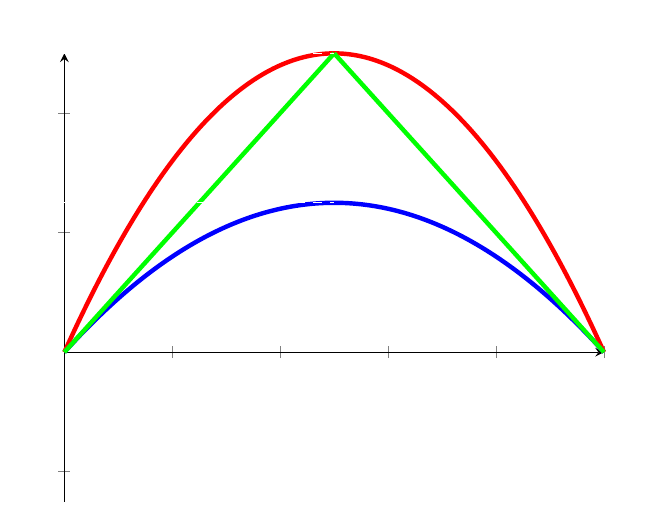
\begin{tikzpicture}[domain=0:1]
           \begin{axis} [ axis lines=center, ymin = -0.25,  yticklabel=\empty, xticklabel = \empty, clip = false]
            
           \addplot[color=blue,samples=100,smooth,ultra thick] {x - x^2};
           \addplot[color=red,samples=100,smooth,ultra thick] {2*x - 2*x^2};
           \addplot[color=green,samples=100,smooth,ultra thick,domain=0:0.5] {x};
           \addplot[color=green,samples=100,smooth,ultra thick,domain=0.5:1] {-x + 1};
        
           \addplot[color = white] coordinates {(1,0)} node[below] {$1$};

            \addplot[color = white] coordinates {(0,0.5)} node[left] {$\frac{1}{2}$};
            \addplot[color = white,dashed] coordinates{(0,0.5) (0.5,0.5)};
            \addplot[color = white,dashed] coordinates{(0,0.25) (0.5,0.25)};
            \addplot[color = white] coordinates {(0,0.25)} node[left] {$\frac{1}{4}$};
        
            \end{axis}
\end{tikzpicture}
}
\begin{enumerate}
\item La parabola più esterna rappresenta $2\alpha(1 - \alpha)$
\item La parabola più interna rappresenta $\alpha(1-\alpha)$
\item In mezzo tra le due \\ $\min{\{\alpha,1-\alpha\}}$ 
\end{enumerate}

\noindent 
Quindi  

$$\frac{|S| |\neg S|}{n} \leq \min{\{\frac{|S|}{n},\frac{|\neg S|}{n}\}}$$

$$\leq 2 \frac{|S| |\neg S|}{n}$$
Ricaviamo che 

$$\phi(S) \leq \frac{n}{d} \sigma(S) \leq 2 \phi(S)$$
per tutti i tagli possibili. Dunque 

$$\phi(G) \leq \frac{n}{d} \sigma(G) \leq 2 \phi(G)$$
possiamo concludere che minimizzare la sparsità è equivalente a minimizzare la conduttanza.

\section{Matrice laplaciana}
Definiamo la \textbf{matrice laplaciana} di un grafo $d$-regolare.  Innanzitutto, sia $A$ la matrice di adiacenza di $G = (V,E)$ dove $A_{ij} = \mathds{I}\{(i,j) \in E\} \in \{0,1\}^{n \times n}$.  La matrice laplaciana $L$ è definita come 

$$L= I - \frac{A}{d}$$
dove
$$(\frac{A}{d})_{ij} = \frac{1}{d} \mathds{I} \{(i,j) \in E\}$$
Per ogni $x \in R^n$ vale che

$$x^T L x = x^T I x - \frac{1}{d} x^T A x$$
sappiamo che $x^t I x = x^T x = ||x||^2 = \sum_{i \in V} x_i^2$

$$\sum_{i \in V} x_i^2 - \frac{1}{d} \sum_{i \in V}\sum_{j \in V} x_i A_{ij} x_j$$ 
Sappiamo che $A_{ij} = 0$ se $(i,j) \notin E$ e attraverso qualche manipolazione algebrica otteniamo

$$= \frac{1}{d} \sum_{i \in V}\sum_{j: (i,j) \in E} x_i^2 - \frac{1}{d} \sum_{i in V} \sum_{j: (i,j) in E} x_i x_j$$

$$= \frac{1}{d} \sum_{i \in V}\sum_{j: (i,j) \in E} (x_i^2 - x_i x_j)$$
Notiamo che stiamo prendendo due volte ogni arco $i,j$. La prima volta con $i$ e la seconda con $j$. Quindi eliminiamo la prima sommatoria, aggiungiamo $x_j^2$ (dato che ci spostiamo solo sugli archi adesso) e raddoppiamo $-x_ix_j$ per contarlo due volte come prima:

$$= \frac{1}{d} \sum_{j: (i,j) \in E} (x_i^2 + x_j^2 - 2x_i x_j)$$

$$= \frac{1}{d} \sum_{j: (i,j) \in E} (x_i - x_j)^2$$
Che è sempre non negativo.  Questo vuol dire che la matrice laplaciana è positiva semidefinita.

\chapter{Undicesima lezione}

\section{Legame matrice laplaciana e autovalori}

\noindent 
Nella scorsa lezione abbiamo scoperto che la matrice laplaciana $L$ è positiva semidefinita. Questo implica che ha $n$ autovalori tali che $0 \leq \lambda_1 \leq \dots \leq \lambda_n$. Prima di andare a lavorare sulla matrice laplaciana vediamola almeno una volta.

\begin{exmp}
   Sia $G=(V,E)$ un grafo $2$-regolare:
    \disegna{
        \node[nodo] (A) at (-1,0) {};
        \node[] at (-1,0.3) {$1$};
        \node[nodo] (B) at (1,0) {};
        \node[] at (1,0.3) {$2$};
        \node[nodo] (C) at (-1,-2) {};
        \node[] at (-1,-2.3) {$3$};
        \node[nodo] (D) at (1,-2) {};
        \node[] at (1,-2.3) {$4$};

        \draw[] (A) -- (B);
        \draw[] (A) -- (C);
        \draw[] (C) -- (D);
        \draw[] (D) -- (B);
    }

    \noindent 
    La matrice d'adiacenza è $A$ è

    \[\mathbf{A} = 
    \bordermatrix{ & 1 & 2 & 3 & 4 \cr
      1 & 0 & 1 & 1 & 0  \cr
      2 & 1 & 0 & 0 & 1  \cr
      3 & 1 & 0 & 0 & 1  \cr 
      4 & 0 & 1 & 1 & 0 } \qquad
      \]
      Da questa otteniamo la matrice laplaciana $L$

      \[\mathbf{L} = 
    \bordermatrix{ & 1 & 2 & 3 & 4 \cr
      1 & 1 & -\frac{1}{2} & -\frac{1}{2} & 0  \cr
      2 & -\frac{1}{2} & 1 & 0 & -\frac{1}{2}  \cr
      3 & -\frac{1}{2} & 0 & 1 & -\frac{1}{2}  \cr 
      4 & 0 & -\frac{1}{2} & -\frac{1}{2} & 1 } \qquad
      \]
\end{exmp}

\noindent 
In generale, una matrice laplaciana è tale che la somma sulle righe  è $= 0$ e la somma sulle colonne è $= 0$. Prendiamo il primo autovalore

$$\lambda_1 = \min_{U \in \mathbb{R} \backslash 0} \frac{U^T L U}{U^T U}$$
Sappiamo che $\lambda_1 \geq 0$ perché $L$ è positiva semidefinita. Definiamo il vettore $\mathds{1} = (1,\dots,1) \in \mathbb{R}^n$ ovvero il vettore contenente tutti $1$. Allora 

\[
L \cdot \mathds{1} = \begin{bmatrix}
        \sum_{j = 1}^n L_{1j}\\ 
        \vdots \\
        \sum_{j = 1}^n L_{nj}
\end{bmatrix} = \begin{bmatrix}
        0\\ 
        \vdots \\
        0
        \end{bmatrix}
\]
Quindi $\mathds{1}^T L \mathds{1} = 0$. Quindi $\lambda_1 = 0$ dato che $0$ è il minimo valore possibile ottenibile ed esiste un vettore, ovvero $\mathds{1}$ tale per cui il coefficiente di Rayleigh è $0$. Per il teorema spettrale $U_1 = \frac{\mathds{1}}{\sqrt{n}}$ (dove $\sqrt{n}$ serve a normalizzarlo) è un autovettore con autovalore $\lambda_1 = 0$. 
Ogni altro autovettore $U$ è tale che $$U^T \frac{\mathds{1}}{n} = 0 \leftrightarrow U^T \mathds{1} = 0 \leftrightarrow \sum_{i = 1}^n u_i = 0$$
Concentriamoci sul secondo autovalore, $\lambda_2$. Vale che 

$$\lambda_2 = \min_{\substack{U \in \mathbf{R}^n \backslash \{0\} \\ U^T \perp \mathds{1} = 0 }} \frac{U^T L U}{U^T U}$$

$$= \min_{\substack{U \in \mathbf{R}^n \backslash \{0\} \\ U^T \perp \mathds{1} = 0 }} \frac{\sum_{(i,j) \in E} (u_i - u_j)^2}{d \sum_{i \in V} u_i^2}$$
Se $G$ ha due componenti connesse

\disegna{
    \node[cloud,draw,minimum width = 2.5cm,
    minimum height = 3cm] at (-1.5,0) {$X$};
    \node[cloud,draw,minimum width = 2.5cm,
    minimum height = 3cm] (A) at (1.5,0){$Y$};
 }

 \noindent 
 Scegliamo  $U \in \mathbb{R}^n$ tale che 

$$u_i = \begin{cases}
    \frac{1}{|X|} \hspace{20px} \text{se}\; i \in X \\
    \frac{1}{|Y|} \hspace{20px} \text{se}\; i \in Y 
\end{cases}$$
Vale che $U^T \mathds{1} = 0$. Infatti, per  \\ $\sum_x u_i = 1$ e $\sum_y u_i = -1$, quindi $\sum_x u_i + \sum_y u_1 = 0$. Inoltre $U^T L U = 0$ perché:

\begin{itemize}
    \item Se $i,j \in X$ allora $u_i - u_j = 0$.
    \item Se $i,j \in Y$ allora $u_j - u_j = 0$.
    \item Non può esistere il caso in cui $i \in X, j \in Y$ o viceversa.
\end{itemize}

\noindent
Quindi $\frac{U}{||U||}$ è un autovettore di $G$ con autovalore $0$. Più in generale possiamo affermare che che $\lambda_k = 0$ se $G$ ha $k$ componenti connesse. Questo ci permette di ricavare il numero di componenti connesse di $G$ guardano il numero di autovalori pari a $0$.
Vediamo cosa succede con $\lambda_n$. 

$$\lambda_n = \max_{U \in \mathbb{R}^n \backslash \{0\}} \frac{U^T L U }{U^T U} = \max \frac{\sum_{(i,j) \in E} (u_i - u_j)^2}{d \sum_{i \in V} u_i^2}$$

$$= \max \frac{1}{d \sum u_i^2} \sum_{(i,j) \in E} (u_i^2 + u_j^2 - 2u_iu_j)$$
Sapendo che ogni nodo appare come estremo in $d$ archi distinti

$$= \max \frac{1}{d \sum u_i^2} (d \sum_i u_i^2 -  \sum_{(i,j) \in E} (2u_iu_j
)) $$
sommiamo e sottraiamo $d \sum_i u_i^2$

$$= \max \frac{1}{d \sum u_i^2} (2d \sum_i u_i^2 - (d \sum_i u_i^2 +  \sum_{(i,j) \in E} (2u_iu_j
)) $$

$$= \max 2  - \frac{\sum_{(i,j) \in E} (u_i + u_j)^2}{d \sum_i u_i^2} $$

$$= 2 - \min \frac{\sum_{(i,j) \in E} (u_i + u_j)^2}{d \sum_i u_i^2} $$
Quindi $0 \leq \lambda_n \leq 2$. Notiamo che $\lambda_n$ vale $2$ nel caso in cui nel grafo sia presente una componente bipartita. 
\disegna{
    \node[cloud,draw,minimum width = 2.5cm,
    minimum height = 3cm] at (0,-2) {};
    \node[nodo] (X1) at (-1,2) {};
    \node[nodo] (X2) at (-1,1) {};
    \node[nodo] (X3) at (-1,0) {};
    \node[nodo] (Y1) at (1,2) {};
    \node[nodo] (Y2) at (1,1) {};
    \node[nodo] (Y3) at (1,0) {};
    
    \draw[-] (X1) -- (Y2);
    \draw[-] (X1) -- (Y3);
    \draw[-] (X2) -- (Y1);
    \draw[-] (X2) -- (Y2);
    \draw[-] (X3) -- (Y1);
    \draw[-] (X3) -- (Y3);
 }

 \noindent 
Costruiamo l'autovettore $U \in \mathbb{R}^n$

$$u_i = \begin{cases}
    1  \hfill \text{se}\; i \in X \\
   -1 \hfill \text{se}\; i \in Y  \\
   0 \hspace{20px} \text{altrimenti}
\end{cases}$$
Quindi $\sum_{(i,j) \in E} (u_i + u_j)^2 = 0$ e allora $\lambda_n = 0$. 

\section{Disuguaglianza di Cheeger}

Come si lega la sparsità, o la conduttanza, allo spettro?

\begin{defi}
    La disuguaglianza di \textbf{Cheeger} ci dà un'approssimazione di $\phi(G)$:

    $$\frac{\lambda_2}{2} \leq \phi(G) \leq \sqrt{2 \lambda_}$$
\end{defi}
La disuguaglianza di Cheeger può essere anche scritta come

$$\frac{2 \lambda_2}{2n} \leq \sigma(G) \leq \frac{2d}{n} \sqrt{2\lambda_2}$$

\begin{dimo}
Cominciamo a dimostrare la parte sinistra, ovvero $$\frac{\lambda_2}{2} \leq \phi(G)$$
Consideriamo $U \in \mathbb{R}^d $ tale che $U^T \mathds{1} = 0$.

$$\sum_i \sum_j (u_i - u_j)^2 = \sum_i \sum_j (u_i^2 + u_j^2 - 2u_i u_j)$$
$$= n \sum_i u_i^2 + n \sum_j u_j^2 - 2 \sum_i \sum_j u_i u_j$$
Sapendo che $(\sum_i u_i)^2 = (\sum_i u_i) (\sum_j u_j) = \sum_i \sum_j u_i u_j$ scriviamo

$$= 2n \sum_i u_i^2 - 2(\sum_i u_i)^2  = 2n \sum_i u_i^2 - 2(U^T \mathds{1})^2 $$
dato che $U^T \mathds{1} = 0$
$$= 2n \sum_i u_i^2$$
Quindi abbiamo che 

$$\lambda_2 = \min_{\substack{U \in \mathbb{R}^n \backslash \{0\} \\ U^T \mathds{1} = 0}} \frac{\sum_{(i,j) \in E} (u_i - u_j)^2}{d \sum u_i^2} $$
Se $U \neq 0$ e $U^T \mathds{1} = 0$ allora $U \neq 0$ e $U \neq \mathds{1}$. Inoltre usiamo il fatto che $\sum_i u_i^2 = \frac{1}{2n} \sum_{ij} (u_i-u_j)^2$

$$= \min_{\substack{U \in \mathbb{R}^n \backslash \{0, \mathds{1}\}}} \frac{\sum_{(i,j) \in E} (u_i - u_j)^2}{\frac{d}{2n} \sum_{ij} (u_i-u_j)^2}$$
Sia $\forall S \subseteq V, \; U \in \{0,1\}^n$ tale che $u_i = 1 \leftrightarrow i \in S$ ( o in altre parole $u_i = \mathds{I}\{i \in S\}$). Allora 

$$|E(S,\neq S)| = \sum_{(i,j) \in E}(u_i-u_j)^2$$
e sapendo che $u_i = u_i^2$ (dato che $1^2 = 1$ e $0^2 = 0$) possiamo dire

$$|S| |\neg S| = (\sum_i u_i^2) (n-\sum_i u_i^2)$$

$$= n \sum_i u_i^2 - \sum_{i,j} u_i u_j$$
In una dimostrazione precedente avevamo trovato che 
$\sum_i \sum_j (u_i - u_j)^2 = 2n \sum_i u_i^2 - 2(\sum_i u_i)^2$. Il lato destro è esattamente quello che abbiamo noi moltiplicato per un fattore $2$, quindi

$$= \frac{1}{2} \sum_{i,j} (u_i - u_j)^2$$
Allora 

$$\sigma(G) = \min_{(S,\neg S)\; cut} \frac{|E(S,\neg S)|}{|S| |\neg S|}$$

$$= \min_{\substack{U \in \mathbb{R}^n \backslash \{0, \mathds{1}\}}} \frac{\sum_{(i,j) \in E} (u_i - u_j)^2}{\frac{d}{2n} \sum_{ij} (u_i-u_j)^2} \geq \frac{d}{n} \lambda_2$$
Che implica che 

$$\frac{d}{n} \lambda_2 \leq \sigma(G) \leq \frac{2d}{n} \phi(G)$$
Quindi abbiamo dimostrato che 

$$\frac{\lambda_2}{2} \leq \phi(G)$$

\end{dimo}



\end{document}
